%% EU FET Open  Proposal LaTeX template
%% Based on the h2020proposal.cls LaTeX class for writing EU H2020 RIA proposals.
%% 
%% Copyright (c) 2010, Giacomo Indiveri
%%
%%  This latex class is free software: you can redistribute it and/or modify
%%  it under the terms of the GNU General Public License as published by
%%  the Free Software Foundation, either version 3 of the License, or
%%  (at your option) any later version.
%%
%%  h2020proposal.cls is distributed in the hope that it will be useful,
%%  but WITHOUT ANY WARRANTY; without even the implied warranty of
%%  MERCHANTABILITY or FITNESS FOR A PARTICULAR PURPOSE.  See the
%%  GNU General Public License for more details.
%%
%%  You should have received a copy of the GNU General Public License
%%  along with Foobar.  If not, see <http://www.gnu.org/licenses/>.
%%
%%
%% Contributors: Elisabetta Chicca
%%
%% Disclaimer: The template is based on the document provided by the EU Participants Portal 
%% at the address: http://ec.europa.eu/research/participants/data/ref/h2020/call_ptef/pt/h2020-call-pt-ria-ia_en.pdf
%%
%% Use the original source and the http://ec.europa.eu/ documentation for reference. We make no
%% representations or warranties of any kind, express or implied, about the completeness, accuracy,
%% reliability, suitability or availability with respect to the original template.
%% In no event will we be liable for any loss or damage including without limitation, indirect or
%% consequential loss or damage, or any loss or damage whatsoever arising out of, or in connection
%% with, the use of this template and/or class.
%%
%% Makes use of the memoir class. Read the optimum memman documentation for
%% info on how to customize your proposal.


\documentclass[]{h2020proposal}     % Remove 'draft' option for final version
%\documentclass[draft]{h2020proposal}

% For in-line comments use:
% \marginpar{comment text}

%% Extra Packages
%% ========
%\usepackage{fontspec}% Latin Modern by default with xelatex

%% LaTeX Font encoding -- DO NOT CHANGE
%\usepackage[OT1]{fontenc} % Not needed with xelatex

%% Input encoding 'utf8'. In some cases you might need 'utf8x' for
%% extra symbols. Not all editors, especially on Windows, are UTF-8
%% capable, so you may want to use 'latin1' instead.
%\usepackage[utf8]{inputenc} % Not needed with xelatex

%% Babel provides support for languages.  'english' uses British
%% English hyphenation and text snippets like "Figure" and
%% "Theorem". Use the option 'ngerman' if your document is in German.
%% Use 'american' for American English.  Note that if you change this,
%% the next LaTeX run may show spurious errors.  Simply run it again.
%% If they persist, remove the .aux file and try again.
\usepackage[english]{babel}

%% For underlined wrapped text.
\usepackage{soul}

%% This changes default fonts for both text and math mode to use Herman Zapfs
%% excellent Palatino font.  Do not change this.
%\usepackage[sc]{mathpazo} % Not needed with xelatex

%% The AMS-LaTeX extensions for mathematical typesetting.  Do not
%% remove.
\usepackage{amsmath,amssymb,amsfonts,mathrsfs}

%% Gantt Charts in LaTeX
\usepackage{pgfgantt}

%% LaTeX' own graphics handling
\usepackage{graphicx}

%% Fancy character protrusion.  Must be loaded after all fonts.
\usepackage[activate]{pdfcprot}

%% Nicer tables.  Read the excellent documentation.
\usepackage{booktabs}

% Compressed itemized lists (with a * at the end)
\usepackage{mdwlist}

%% Nicer URLs.  
\usepackage{url}

%% Configure citation styles
\usepackage[numbers,sort&compress,square]{natbib}
\def\bibfont{\footnotesize}     %for smaller fonts in the biblio section

%% Hyper Ref package. In order to operate correctly, it must be the last package declared
\usepackage[colorlinks,pagebackref,breaklinks]{hyperref} 

\usepackage{marvosym}

%% Extra package options
\hypersetup{pdftitle={Completeness of the Gaia-verse, CoG}, pdfsubject={RIA in SPACE-30-SCI-2020: Scientific data exploitation}, pdfauthor={A.G.A. Brown, H.W. Rix, M. Fouesneau, R. Drimmel, V. Belokurov, A. Casey, D. Hogg},
  hypertexnames=true, linkcolor=blue, anchorcolor=black,
  citecolor=blue, urlcolor=blue  
}

\urlstyle{rm} %so it doesn't use a typewriter font for urls.
\DeclareGraphicsExtensions{.jpg,.pdf,.mps,.png} % for pdflatex
\graphicspath{{img/} {./}} %put all figures in these dirs

\newcommand*\aap{A\&A}
\let\astap=\aap
\newcommand*\aapr{A\&A~Rev.}
\newcommand*\aaps{A\&AS}
\newcommand*\actaa{Acta Astron.}
\newcommand*\aj{AJ}
\newcommand*\ao{Appl.~Opt.}
\let\applopt\ao
\newcommand*\apj{ApJ}
\newcommand*\apjl{ApJ}
\let\apjlett\apjl
\newcommand*\apjs{ApJS}
\let\apjsupp\apjs
\newcommand*\aplett{Astrophys.~Lett.}
\newcommand*\apspr{Astrophys.~Space~Phys.~Res.}
\newcommand*\apss{Ap\&SS}
\newcommand*\araa{ARA\&A}
\newcommand*\azh{AZh}
\newcommand*\baas{BAAS}
\newcommand*\bac{Bull. astr. Inst. Czechosl.}
\newcommand*\bain{Bull.~Astron.~Inst.~Netherlands}
\newcommand*\caa{Chinese Astron. Astrophys.}
\newcommand*\cjaa{Chinese J. Astron. Astrophys.}
\newcommand*\fcp{Fund.~Cosmic~Phys.}
\newcommand*\gca{Geochim.~Cosmochim.~Acta}
\newcommand*\grl{Geophys.~Res.~Lett.}
\newcommand*\iaucirc{IAU~Circ.}
\newcommand*\icarus{Icarus}
\newcommand*\jcap{J. Cosmology Astropart. Phys.}
\newcommand*\jcp{J.~Chem.~Phys.}
\newcommand*\jgr{J.~Geophys.~Res.}
\newcommand*\jqsrt{J.~Quant.~Spectr.~Rad.~Transf.}
\newcommand*\jrasc{JRASC}
\newcommand*\memras{MmRAS}
\newcommand*\memsai{Mem.~Soc.~Astron.~Italiana}
\newcommand*\mnras{MNRAS}
\newcommand*\na{New A}
\newcommand*\nar{New A Rev.}
\newcommand*\nat{Nature}
\newcommand*\nphysa{Nucl.~Phys.~A}
\newcommand*\pasa{PASA}
\newcommand*\pasj{PASJ}
\newcommand*\pasp{PASP}
\newcommand*\physrep{Phys.~Rep.}
\newcommand*\physscr{Phys.~Scr}
\newcommand*\planss{Planet.~Space~Sci.}
\newcommand*\pra{Phys.~Rev.~A}
\newcommand*\prb{Phys.~Rev.~B}
\newcommand*\prc{Phys.~Rev.~C}
\newcommand*\prd{Phys.~Rev.~D}
\newcommand*\pre{Phys.~Rev.~E}
\newcommand*\prl{Phys.~Rev.~Lett.}
\newcommand*\procspie{Proc.~SPIE}
\newcommand*\qjras{QJRAS}
\newcommand*\rmxaa{Rev. Mexicana Astron. Astrofis.}
\newcommand*\skytel{S\&T}
\newcommand*\solphys{Sol.~Phys.}
\newcommand*\sovast{Soviet~Ast.}
\newcommand*\ssr{Space~Sci.~Rev.}
\newcommand*\zap{ZAp}

\newcommand\memo[1]{\textcolor{red}{\textbf{#1}}}
% Duration of project in months. For now assumed 6 months preparation (hiring etc) and 36 months actual work.
\newcommand\duration{42}
\newcommand\acro{CoG}
\newcommand\equref[1]{equation (\ref{#1})} 
\newcommand\equrefcap[1]{Equation (\ref{#1})} 
\newcommand\figref[1]{figure \ref{#1}}
\newcommand\figrefs[1]{figures \ref{#1}}
\newcommand\figrefcap[1]{Figure \ref{#1}}
\newcommand\figrefscap[1]{Figures \ref{#1}}
\newcommand\tabref[1]{table \ref{#1}}
\newcommand\tabrefcap[1]{Table \ref{#1}}
\newcommand\secref[1]{section \ref{#1}}
\newcommand\secrefcap[1]{Section \ref{#1}}
\newcommand\apref[1]{appendix \ref{#1}}
\newcommand\aprefcap[1]{Appendix \ref{#1}}
\newcommand{\By}[2]{ {\textcolor{orange}{ #1 :}} {\textcolor{blue}{ #2}}}
\newcommand{\given}{\ensuremath{\mid}}
\newcommand{\pem}{person-month}
\newcommand{\pems}{person-months}

%%%%%%%%%%%%%%%%%%%%%%%%%%%%%%%%%%%%%%%%%%%%%%%%%%%%%%%%%%%%%%%%%%%%%%

%% ========================================================
%% IMPORTANT store proposal information in global variables
%% ========================================================
\title{Completeness of the Gaia-verse\\ \memo{(working title and acronym: other suggestions welcome)}
\\ \memo{Who is In, and Who is Not? \\ Determining the Gaia Data's Selection Function}}
% ARC suggests: Completeness of the Cosmos?
%               (obvious down-side is that there's no Gaia in the title)
\shortname{\acro} 
\titlelogo{}{0.25} % file name and scale
\fundingscheme{Research and Innovation Action}
\topic{SPACE-30-SCI-2020: Scientific data exploitation}
\coordinator{Anthony G.A.~Brown}{brown@strw.leidenuniv.nl}{Universiteit Leiden}
\participant{Universiteit Leiden}{ULEI}{Netherlands} % First participant is the coordinator
\participant{Max-Planck-Institut f\"ur Astronomie}{MPIA}{Germany} % as example...
\participant{Osservatorio Astrofisico di Torino}{INAF}{Italy} % as example...
\participant{University of Cambridge}{UCAM}{United Kingdom}
\participant{Monash University}{MONA}{Australia}
\participant{New York University}{NYU}{United States}
% etc.

% Page Headers
%\makeoddhead{proposal}{\disptoken{@acronym}}{}{\rightmark}
%\makeevenhead{proposal}{\leftmark}{}{\disptoken{@acronym}}

%Page Footers
%\makeevenfoot{proposal}{ \thepage }{ \date{\today} }{ \disptoken{@acronym} }
%\makeoddfoot{proposal}{  }{ \date{\today} }{ \thepage }

%Page Style
\pagestyle{proposal} %use \pagestyle{showlocs} for debugging

%Heading style 
\makeheadstyles{default}{%
\renewcommand*{\chapnamefont}{\normalfont\bfseries}
\renewcommand*{\chapnumfont}{\normalfont\bfseries}
\renewcommand*{\chaptitlefont}{\normalfont\bfseries}
\renewcommand*{\secheadstyle}{\normalfont\bfseries}
}%
\headstyles{default}

%Chapter Style
\chapterstyle{section} %Avoid writing the word "Chapter" at the beginning of each proposal section
% other possible valid styles:
% article, bringhurst, crosshead, culver, dash, demo2, ell, southall, tandh, verville, wilsondob
\renewcommand*{\chaptitlefont}{\normalfont\Large\bfseries}
\renewcommand*{\chapnumfont}{\normalfont\Large\bfseries}

\begin{document}

\maketitle
%\vspace{-4em}
\renewcommand\contentsname{\normalsize Table of Contents \vspace{-4em}}
\setlength{\cftbeforechapterskip}{1.0em plus 0.3em minus 0.1em}
\renewcommand{\cftchapterbreak}{\addpenalty{-4000}}
\makeparticipantstable          %for the ICT RIA proposals
\tableofcontents*               %for the ICT RIA proposals
%\begin{abstract}
  Project abstract. \textbf{Important:} limit to 2000 characters. 
\end{abstract}
\thispagestyle{empty}
\pagebreak

%%% Important. To have correct table numberings
\renewcommand{\thetable}{\thesection\alph{table}}

\chapter[Excellence]{Excellence}
\label{cha:excellence}
\instructions{
Your proposal must address a work programme topic for this call for proposals. \\
\textit{This section of your proposal will be assessed only to the extent that it is relevant to that topic.}\\
}

\section{Objectives}
\label{sec:objectives}
\instructions{
Describe the overall and specific objectives for the project1, which should be clear, measurable,
realistic and achievable within the duration of the project. Objectives should be consistent with
the expected exploitation and impact of the project (see section 2).
}

The European Space Agency's Gaia Mission \cite{2016A&A...595A...1G} is the most successful of ESA's space astronomy missions as measured by the publication rate of papers using its data in one form or another. Over 2500 papers appeared between April 2018 and February 2020 that use data from the second Gaia data release\footnote{As indicated for example by the \href{https://ui.adsabs.harvard.edu/search/q=citations(bibcode\%3A2018A\%26A...616A...1G)&sort=date\%20desc\%2C\%20bibcode\%20desc&p_=0}{citations to the Gaia DR2 release paper}}. Among the many high profile science results published by European groups are the discovery of a spiral in the phase space structure of the Milky Way's disk (\cite{2018Natur.561..360A} indicative of a recent disturbance, most likely due to the Sagittarius dwarf galaxy), the first direct observational evidence of crystallization in the interiors of white dwarfs \cite{2019Natur.565..202T} (confirming a fifty year old prediction), and the uncovering of a major event 10 billion years into the Milky Way's past when a collision with a dwarf galaxy took place which contributed to the build-up of the Milky Way's stellar halo and thick disk \cite{2018Natur.563...85H, 2018MNRAS.478..611B, 2019arXiv190904679B}. 

But while there are numerous exciting results that are starting to transform many different fields of astrophysics, it remains true that most of these to date have focused on `low hanging fruit' in the Gaia data archive, and barely scratched the surface of the Gaia data information content. Specifically, almost all analyses to date have exploited the astounding Gaia data precision and accuracy on all the individual objects, but have side-stepped performing or exploiting the \textsl{statistical distribution of objects with certain properties}, i.e. population studies. For example, a result as elementary as a good determination of the Milky Way's radial profile of disk stars -- by simply counting them as a function of their position -- has yet to be carried out.  This is because such studies inevitably require knowledge of the ``selection function'': what is the probability that an object of certain physical properties at a certain position in space would be catalogued by Gaia? This knowledge is indispensible for any population study of objects; and population studies are the very core of the Gaia mission, with its billions-of-objects catalogue.

In practice the community so far has often resorted to drastic cuts, on object properties and Gaia data quality flags, to arrive at samples whose selection function is very simple (avoiding for example the well known problems associated with the estimation of distance as the inverse of the parallax \cite{2018A&A...616A...9L}). Yet, such analyses grossly under-exploit the information content of the Gaia data set, often by orders of magnitude.

Consequently, many high-profile science cases for which Gaia was built cannot be realized, because the selection function of the Gaia survey is not known, neither to the Gaia DPAC team, nor to the community. When  combined with the some additional data cuts, this leads to unrepresentative samples. It is the single goal of this proposal to remedy this shortcoming and dramatically boost (yes, yet further!) the astrophysical utility of the Gaia mission.

The Gaia selection function is a highly non-trivial combination of the on-board selection of sources, telemetry losses, selections on data quality during processing, and selections on quality before the publication of the processed data in the Gaia archive. As a result, the selection function for Gaia has only been characterized in highly simplified ways \memo{(provide literature references in the motivation section below)} even though it will be crucial for a full exploitation of the intrinsic science potential of the Gaia data, in particular also in view of the legacy value of the Gaia archive which will remain the standard in fundamental astrophysical data for decades to come.

The objective of this proposal is to build a detailed selection function for the Gaia data and to provide this to the scientific community in the form of numerical tables and source code that allow users to apply the selection function to their scientific analyses and thus maximize the outcome thereof. In detail the objectives are:

\begin{enumerate}
    \item Develop a detailed mathematical formulation of a survey selection function, where the goal is to keep this as general as possible even if in this project the focus is on the Gaia survey. The formulation should account for the layering of user imposed sample selections on top of the survey selection function and allow for a description of the selection function of combinations of surveys.
    \item Research and develop a detailed description and modelling of the Gaia survey selection function and do the same for the combination of Gaia and other surveys. The results will set the requirements for the next two items.
    \item Provide a detailed practical implementation of the Gaia selection function in the form of auxiliary data, which will be accessible through the ESA Science Data Centre, and open source tools which will be made available through code hosting websites. 
    \item Develop tools to incorporate the selection function in scientific analyses. These tools should allow for combining the Gaia survey selection function with user imposed sample restrictions and for combining Gaia with other surveys. The tools will be made available as open source code through code hosting websites.
    \item Apply the selection function tools to example science cases. This will serve to demonstrate the benefits of carefully accounting for the selection function and at the same time provide worked examples to the community of prospective users of these tools.
\end{enumerate}

The long term curation of the results will be ensured through the availability of the auxiliary data through the ESA Gaia archive and by source code for the uers tools being embedded in or affiliated to the Astropy project.

\subsection{Context}
\label{sec:context}

ESA's Gaia mission \cite{2016A&A...595A...1G} represents a European breakthrough in astrophysics, a cornerstone mission which was launched in 2013 aimed at producing the most accurate 3D map of the Milky Way to date. The resulting stereoscopic census of our Galaxy represents a giant leap in astrometric accuracy (reaching the 10--20 micro-arcsecond regime, which is equivalent to knowing the 3D positions of stars to 10 per cent precision over distances as large as $20\,000$ to $30\,000$ light-years) complemented by the only full sky homogeneous photometric survey with an angular resolution comparable to that of the Hubble Space Telescope, as well as the largest spectroscopic survey ever undertaken. 

The primary scientific aim of the mission is to map the structure of our Galaxy and unravel its formation history and subsequent evolution. Current cosmological models envisage the formation of large galaxies through the merging of smaller structures. Deciphering the assembly history of our Galaxy requires a detailed mapping of the structure, dynamics, chemical composition, and age distribution of its stellar populations. Ideally one would like to `tag' individual stars to each of the progenitor building blocks of the Galaxy \cite{2002ARA&A..40..487F}. The Gaia mission is designed to provide the required fundamental data in the form of distances (through parallaxes), space velocities (through proper motions and radial velocities) and astrophysical characterisation (through multi-colour photometry) for massive numbers of stars throughout most of the Galaxy. It should be stressed however that Gaia is not simply a `Milky Way mission' but is truly a multi-faceted {\em astrophysics mission} which will provide exciting scientific results covering many topics including: fundamental stellar physics across the Hertzsprung-Russell diagram, the characterisation of tens of millions of binary stars, unique samples of variable stars of nearly all types (including key cosmological distance calibrators), detection and orbital classification of thousands of exo-planetary systems, a comprehensive survey of objects ranging from huge numbers of minor bodies in our Solar System, through galaxies in the nearby Universe, to over a million distant quasars. Gaia will also provide a number of stringent tests of general relativity. Last but not least, a massive survey such as Gaia will uncover many surprises that the Universe still holds in store for us.

The data processing for the Gaia mission is carried out by a European consortium of institutes and funding agencies, the Data Processing and Analysis Consortium (DPAC). The task of the DPAC is to turn the raw telemetry from Gaia into data products ready for use by astronomers and scientists around the world. The data products are both the basic astrometric, photometric, and spectroscopic results as well as advanced data products, such as the astrophysical characterization of stars, derived from the former. Through an independent unit within the consortium the DPAC also ensures the quality of the published data through extensive technical and scientific validation. The publicly released data, which are disseminated through the ESA Science Data Center and its partners, are accompanied by extensive documentation which is also produced by DPAC. It should be stressed here that the DPAC holds no proprietary rights to the data which means that once the data products are validated and documented they are released publicly and world-wide without delay. In this sense Gaia represents a uniquely open survey concept.

From the early days of the Gaia mission it was foreseen to have incremental data releases based on increasing amounts of collected telemetry. The various data products would be released in stages (where, for example, some of the advanced data products such as exoplanet catalogues can only be released after sufficient data has been collected and the various astrometric calibrations have reached the required levels of precision) and with increasing accuracy for each release. To date two data releases have taken place, Gaia DR1 in September 2016 and Gaia DR2 in April 2018. Both releases have been highly successful and have had major impacts on the fields of Galactic archaeology; Milky Way mass estimation; stellar streams, dwarf galaxies, globular clusters; open clusters; white dwarfs; the characterization of exoplanet host stars and determining the absolute sizes of protoplanetary disks, to name a number of prominent examples. The studies of individual stars and stellar systems benefit immensely from the now easily available high precision parallax data.

The next releases foreseen are Gaia EDR3 in the third quarter of 2020 and Gaia DR3 in the second half of 2021. The following release (Gaia DR4) will be based on all data collected during the nominal mission lifetime of Gaia and feature the full suite of data products, including the epoch data (individual measurements) for the astrometry, photometry, and spectroscopy\footnote{See the \href{https://www.cosmos.esa.int/web/gaia/release}{Gaia data release scenario} pages.}. These future Gaia data releases are expected to have an even larger impact on astronomy due to the much richer set of data products allowing for the combination of high accuracy astrometry and radial velocities with detailed astrophysical characterization of the source in the Gaia catalogue (stellar parameters including chemical compositions and variability, parameters of multiple stars and exoplanets, medium resolution spectra around the Ca triplet region for millions of stars to magnitude 13, low resolution prism spectrophotometry for all sources in the Gaia catalogue). 

Despite the major successes of Gaia DR1 and Gaia DR2 there is one serious weakness of the releases: the DPAC does not provide a detailed selection function for the Gaia survey. This aspect has never been included in the funded DPAC efforts and will not be added as DPAC work in the future. This implies that major Gaia science cases cannot be addressed by the astronomical community to the full potential of the quality of the data. In \secref{sec:scientific-motivation} we motivate why a detailed selection function is needed and how this will enhance the scientific exploitation of the data from this flagship European space mission. 

\paragraph{Gaia instruments and survey strategy} For the understanding of the work proposed here it is useful to briefly summarize the characteristics of the Gaia mission and how the measurements are collected and subsequently processed on ground. Much more detail can be found in the paper describing the Gaia mission \cite{2016A&A...595A...1G}. The Gaia spacecraft and its instruments were designed to collect data that will allow the determination of highly accurate positions, parallaxes, and proper motions for $>1$ billion sources brighter than magnitude $20.7$ in its white-light photometric band $G$ (covering the range $330$--$1050$~nm). The astrometry is complemented by multi-colour photometry, measured for all sources observed by Gaia, and radial velocities which are collected for stars brighter than $G\approx17$. Gaia carries two telescopes of which the collected light is combined into a single focal plane servicing the three main instruments. The astrometric instrument collects source images in the $G$-band, where the fundamental inputs to the astrometric data processing consist of the precise times when the image centroids pass a fiducial line in the focal plane of the instrument. The photometric instrument is realised through two prisms dispersing the light entering the field of view of two dedicated sets of CCDs. The Blue Photometer (BP) operates over the wavelength range $330$--$680$ nm, while the Red Photometer (RP) covers the wavelength range $640$--$1050$ nm. The data collected by the photometric instrument consists of low resolution spectrophotometric measurements of the source spectral energy distributions. The spectroscopic instrument, also called the radial-velocity spectrometer (RVS), collects medium resolution ($R\sim11\,700$) spectra over the wavelength range $845$--$872$~nm, centred on the Calcium triplet region. The spectra are collected for all sources to $G\approx17$ (16$^\text{th}$ magnitude in the RVS filter band).

The Gaia sky survey strategy is derived from that of the Hipparcos mission and and relies on the spacecraft slowly spinning around the axis perpendicular to the lines of sight of the two telescopes (which are separated by $106.5^\circ$. Every six hours the Gaia telescopes can scan a great circle on the sky with an across scan field of view size of $0.7^\circ$. By slowly precessing the spin axis around the direction to the Sun the full sky can be surveyed with optimal sky coverage uniformity over the five years nominal mission lifetime. 

The processing of the observations collected by Gaia is carried out by the DPAC through a series of complex pipelines which are part of a large iterative system (see section 7 in \cite{2016A&A...595A...1G}).

Although the Gaia survey selection function is seemingly very simple, with only a magnitude limit imposed on the observations (see \figref{fig:gsf_ideal}), each of the above components of the Gaia mission adds complexity to the survey selection function as illustrated in \figref{fig:gsf_realistic}. A few examples are listed here:
\begin{itemize}
    \item The data collection on the spacecraft is limited by the amount of sources that can be handled at any on time, meaning that for dense regions on the sky (above $10^6$, $750\,000$, and $35\,000$ sources~deg$^{-2}$ for the astrometric, photometric, and spectroscopic instruments respectively) not all sources can be measured, leading to brighter effective survey limits in those regions. In addition the on-board storage capacity limitations combined with available ground station time lead to deletion of data on occasions when both Gaia telescopes are scanning along the Galactic plane for prolonged periods of time.
    \item Despite the optimal sky survey strategy realized through the revolving scanning technique, the number of times any given source is observed does vary with celestial position, in particular with the ecliptic latitude.
    \item Decisions are made along each of the various on-ground data processing steps on which data and/or sources to process, where periods of ``bad inputs'' are excluded. This leads to gaps in the time coverage of measurements for a given source or to effectively brighter survey limits covering certain time periods (which translates to certain areas on the sky). Additionally, in early data releases the processing for certain data products may be limited to brighter sources or sources with specific astrophysical characteristics.
\end{itemize}
Each of the above examples complicates the Gaia survey selection function which in the end is very non-trivial to describe and handle. Nevertheless we must make an effort to provide the best possible description of the selection function as well as tools to incorporate it into scientific analyses as we motivate in \secref{sec:scientific-motivation}.

\paragraph{Timing of this proposal} We stress here that the time to research a detailed selection function for the Gaia survey is \emph{now}:
\begin{itemize}
    \item To understand the selection function in detail, accounting for all the issues described above and in \secref{sec:concept}, requires access to the Gaia spacecraft and data processing expertise within DPAC and ESA. It is thus essential to start this work while the DPAC is still active.
    \item Already now the availability of a selection function for the Gaia DR2 catalogue would represent a major boost to the science exploitation of those data.
    \item Which each upcoming Gaia data release the complexities of the selection function will increase thus making any effort postponed to the future much more costly in terms of human resources required.
\end{itemize}

\subsection{Scientific motivation}
\label{sec:scientific-motivation}

\subsubsection{The Selection-Function: Definition and Indispensability} %\By{HWR}{}}
%
%\textbf{Douglas: Apologies, I haven't found time to properly attempt this yet.}
%
%\By{HWR}{putting meat on the subsequent section, drawing on a Hogg\&Rix2020 in prep paper on 'selection functions'}

For any `statistical' study using a catalog, for any study where it matters quantitatively how common or rare a certain type of object or circumstance is, the selection function of a catalog is arguably as important as the catalog itself. The catalog \textit{selection function}, $S_C(y)$, is a function of the observable (and thereby underlying physical) properties, $y$, of any astronomical objects; and it specifies the probability that an object of properties $y$ will enter the (Gaia) catalog. A generic and central way of learning from any catalog, is to envision a set of physical or mathematical models $\lambda_0(z\given\theta)$ -- that predicts the
distribution of true quantities $z$, given a set of model parameters $\theta$ -- and then ask
what the `data' (the catalog entries) $\lambda_C(y\given\theta)$ tell us about the relative plausibility. 
The relation between these quantities is generically
\begin{equation}
\lambda_C(y\given\theta) = S_C(y)\,\int p(y\given z)\,\lambda_0(z\given\theta)\,{\textrm{d}} z = S_C(y)\,\lambda_0(y\given\theta),
\label{eqn:selfunc_definition}
\end{equation}
where $z$ is the vector of true values (\emph{vs.} the observed values $y$). 
\textbf{This immediately shows that no inference, is possible without knowledge of $\mathbf{S_C(y)}$}. Most commonly the quantities $y_s$ on which the selection function really depends is only a modest subset of all the catalog entries, or all the quantities that are being modelled, $y$, the selection function separates $S_C(y_s) \times S_0(y_{other})$, with $S_0(y_{other})\approx 1$. 
For the Gaia catalog selection function, the quantities $y_s$ are (in presumably good approximation): the sky position $(\alpha,\,\delta)$ of an object, its magnitude in the visible G band, and its BP$-$RP color from the spectrophotometric bands.\footnote{For objects with very high proper motions, e.g. in the Solar system, the selection function may also depend on $\vec{\mu}$; this interesting regime, affecting a very small fraction of the Gaia detections, is not the focus of this proposal.} These four quantities are a small subset of the Gaia catalog entries. So, why is it hard to determine a good approximation of the Gaia catalog selection function, $S_C(y_s)$? This is because 
$S_C(y_s)$ is such a complex function of the $y_s$: the sky position enters through the source density (``crowding'') and the scanning pattern, which sets the number of observation epochs and the distribution of roll angles; the roll angle in turn determines the (sky) direction in which the BP, RP and RVS spectra are dispersed, which in turn determines the probability that they are rendered unusable dues to source-source contamination. The magnitudes determine not only the obvious aspect of the photon noise, but -- in conjunction with the source density -- also the decision of parsing the data into postage stamps for processing.

Given that $S_C(y_s)$ has not (yet) been determined for Gaia, why is it that many %results of
widely accepted results have already come from analysing the distribution of Gaia catalog entries for large samples? This is for a number of reasons. First, some studies have essentially ignored (at their own peril) the selection function, thereby implicitly assuming $S_C(y_s)\approx 1$ for the regime of interest. The second and most frequent regime so far is that one can make additional ``sample cuts'' by defining
\begin{equation*}
    S_{cut}(y) = \begin{cases} 1 &\mbox{if\ \ } y \mbox{\ \ within cuts} \\ 
0 &\mbox{\ \ else} \end{cases}
\end{equation*}
If one then models only the restricted data $\lambda_{cut}(y\given\theta)$, Eq.\ref{eqn:selfunc_definition} becomes simple, as one the can sensibly adopt
%as the right hand side can be supposedly approximated as 
\begin{equation*}
    \lambda_{cut}(y\given\theta) \approx S_C(y) \times S_{cut}(y)\, \lambda_0(y\given \theta) \approx  \begin{cases}  \lambda_0(y\given \theta) &\mbox{if\ \ } y \mbox{\ \ within cuts} \\ 
0 &\mbox{\ \ else.} \end{cases}
\end{equation*}
A pertinent example would be that for a 'stellar halo study' $S_{cut}(y)$ limits the analysis to, say, blue-ish (BP$\_$RP$<1$) stars of $13.5<G<17.5$ at high Galactic latitudes, away from Globular clusters and the Magellanic Clouds. Then the assumption that the small sub-sample is nearly complete within the stated $S_{cut}(y)$  is defensible.
%}

The third regime is that one can analyze the distribution of quantities in $p(y_{other})$, or $p(y_{other}~|~y_s)$: the most obvious case is to analyze the 3D kinematic in the Solar neighbourhood. The last regime is of course, that the selection function $S_C(y_s)$ has been ``properly'' determined and included in the modelling [REF]; however this has only happened to date for very small sub-regimes of the space spanned by $y_s$ in the Gaia catalog.


\textbf{It is the comprehensive construction of this (approximate) selection function, $S_C(y_s)$, that is at the heart of this proposal.} As we now sketch with a few examples, without its robust and precise knowledge it is impossible to extrapolate from \textit{statements about the objects' population in a catalog} into \textit{insights in fundamental physics and astrophysics}.

\subsubsection{Highlight Gaia Science that cannot be done without a Good Selection-Function}
We now proceed to highlight a few science cases central to Gaia's scientific success that absolutely require a well-determined selection function to be feasible\footnote{By `feasible' in this context we mean: able to address a science question with a quantitative understanding of the dominant source of systematic uncertainty; and not falling short by more than an order-of-magnitude of the full pertinent information content of the Gaia catalog.}.
To illustrate the kinds of selection effects that can occur in the Gaia data we refer to figures \ref{fig:6dsample}--\ref{fig:bulge}. These figures serve also to reinforce the points made in the following text.
\\

\begin{figure}
    \centering
    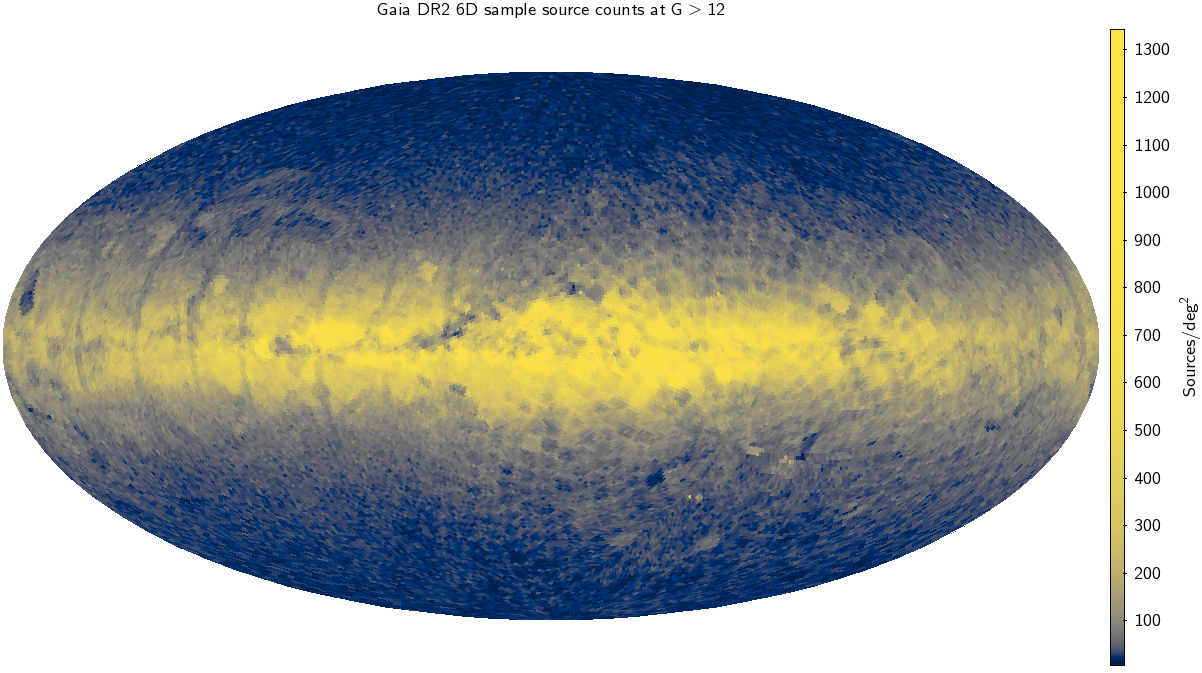
\includegraphics[width=\linewidth]{DR2_6DSample_Source_Counts_Ggt12.png}
    \caption{Source density distribution on the sky (no.\ per square degree) of stars in the Gaia DR2 catalogue for which a radial velocity is listed and which are fainter than $G=12$. The sky projection is in Galactic coordinates with the Milky Way bulge in the centre of the image and the longitude increasing to the left. Note the prominent patterns of squares in the southern hemisphere on the lower right hand side of the figure. These are imprints of photographic plates on which the Guide Star Catalogue is based which was one of the surveys used to construct the Initial Gaia Source List \cite{2014A&A...570A..87S}. This list was used to bootstrap the creation of the Gaia source list (see \secref{sec:methods}). Imprints from the Sloan Digital Sky Survey spectroscopic survey can be seen as dark stripes crossing the Galactic plane on the left hand side. Although these imprints will gradually disappear in future Gaia data releases, this figure is a good illustration of the complications that can arise for selection functions of combined surveys.}
    \label{fig:6dsample}
\end{figure}

\begin{figure}
    \centering
    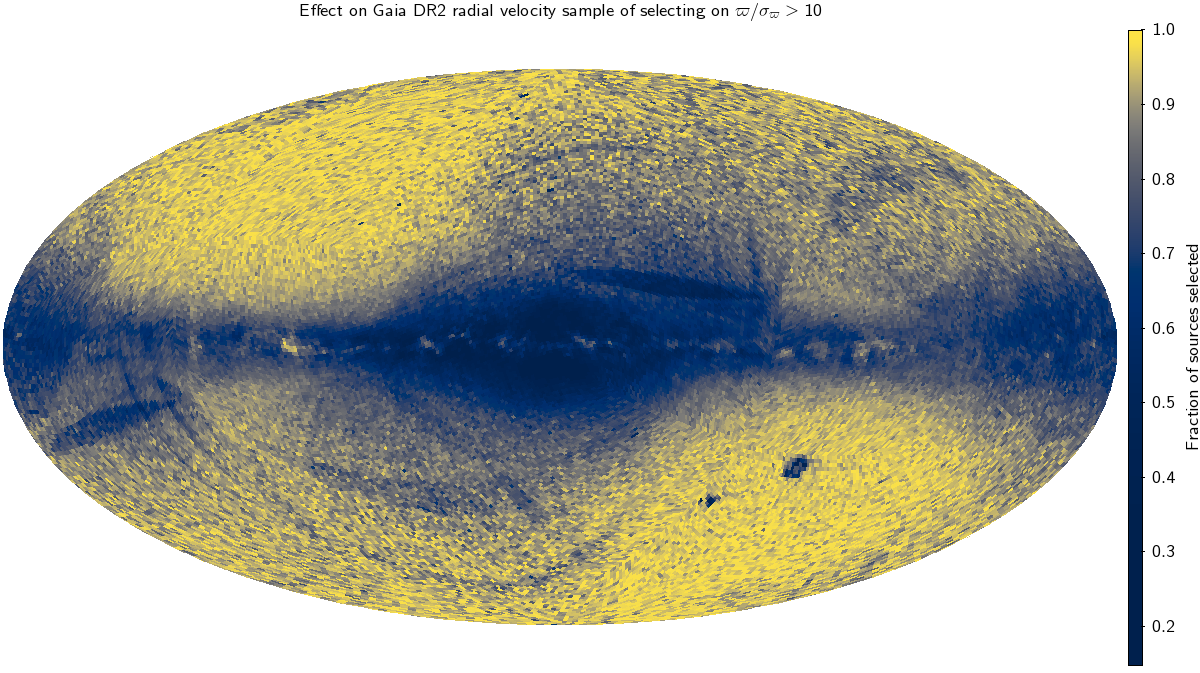
\includegraphics[width=\linewidth]{SelectionEffect6DSamplePlxSnrGt10.png}
    \caption{The fraction of stars selected from the Gaia DR2 sample for which radial velocities are listed, when demanding that the parallax is larger than 10 times its uncertainty. Note how the ecliptic pole regions on the top left and bottom right are strongly favoured, whereas the fraction of selected source drops dramatically along the Galactic plane. In addition there are oddly shaped regions with a lower fraction of selected sources. These reflect a combination of the scanning strategy followed by Gaia and filtering on data quality at various stages in the data processing.}
    \label{fig:6dplxsnrgt10}
\end{figure}
\noindent\textbf{A) 3D-Mapping of the Milky Way}

\begin{figure}
    \centering
    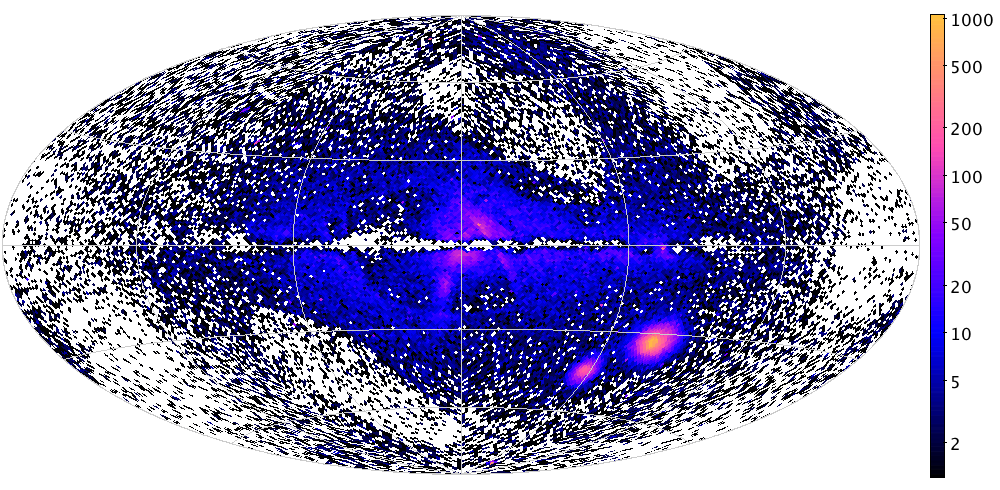
\includegraphics[width=0.7\linewidth]{DR2_skyPlot_sos_RRL_inv.png}
    \caption{The sky distribution of confirmed RR Lyrae variables in the Gaia DR2 catalogue. Note the very strong selection effects on the sky due to the combination of the scanning strategy, the constraints on the minimum number of observations for classifying variable stars, and data quality filtering in the processing pipelines. For details see \cite{2018A&A...618A..30H}.}
    \label{fig:rrl}
\end{figure}

\begin{figure}
    \centering
    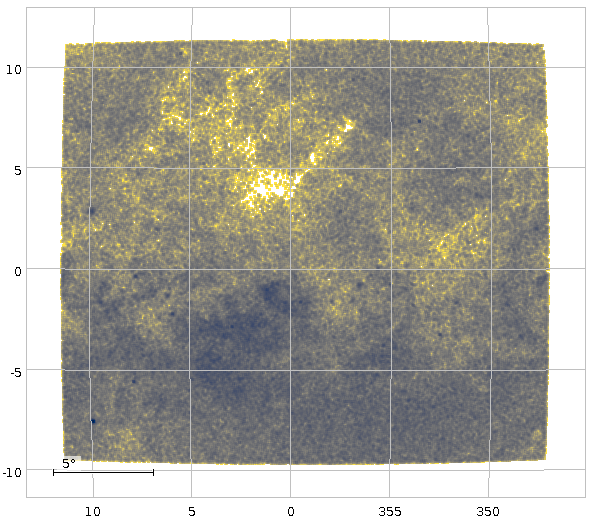
\includegraphics[width=0.5\linewidth]{img/BulgeRegionGlt13.png}\hfil
    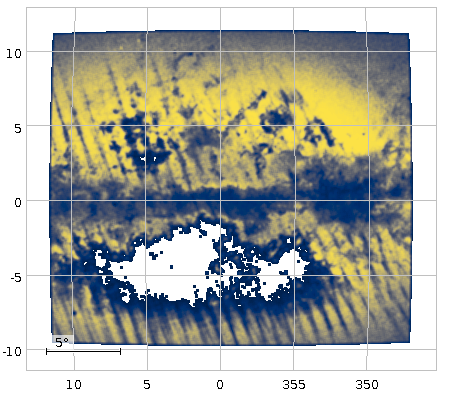
\includegraphics[width=0.5\linewidth]{img/BulgeRegionG20p65to20p70.png}
    \caption{\textbf{Left} The distribution on the sky of sources brighter than $G=13$ (300 thousand sources) in the direction of the Milky Way bulge region. No obvious selection effects are apparent, the darker regions being due to clouds of dust blocking the light from the stars behind them. The white pixels are empty of sources due to severe dust effects.\textbf{Right} The same for sources with $20.65<G<20.70$ (4 million sources). Note the strong striping pattern which again reflects the combination of the Gaia sky scanning strategy and the filtering on data quality during the data processing. The white areas are due to a combination of dust effects and the drop in catalogue completeness at these faint magnitudes.}
    \label{fig:bulge}
\end{figure}

Creating an unprecedented, large-scale 3D map of our Galaxy is arguably the central seminal goal of the Gaia mission, at the heart of setting the fundamental parallax precision science requirements. Yet, to date, no large-scale map of the stellar density (most of which is in the Galactic disk) has emerged. This is because 
such a density map is not merely the combination of the (catalogued) stars distribution $\{y_s\}$, in position, magnitude and color with distances, e.g. from parallaxes. Linking $\{y_s\}$ to $\rho_*(X,Y,Z)$ requires modelling the 3D dust distribution (there are large, coherent efforts underway to do this) and of $S_C(y_s)$. The selection function is so central here, as the quantities to be modelled, are exactly the quantities $y_s$ on which the selection depends!
\\

\noindent\textbf{B) Milky Way Dynamics and Distribution of (Dark) Matter}

Inferring the (dark) mass distribution, or the gravitational potential, in and around our Galaxy from modelling the 6D phase-space distribution of stars is another seminal and central science case for the overall Gaia mission. There are many sophisticated approaches to 'dynamical modelling', but the indispensable role of a well-understood selection function of the stars that serve as kinematic tracers can be illustrated with the arguably simplest form of dynamical modelling, the Jeans Equation. Consider the disk dynamics in the vertical direction (the `Oort limit'):
\begin{equation}
    \frac{\partial[\rho_*(R,z) \overline{v_z^2}(R,z)]}{\partial z}~+~\frac{1}{R}
    \frac{\partial[R \rho_* \overline{v_z v_R}]}{\partial R} + \rho_*\frac{\Phi(R,z)}{\partial z}=0 \mathrm{\ or\ \ } \frac{\partial[\rho_*(R,z) \overline{v_z^2(R,z)}]}{\partial z} + \rho_*\frac{\Phi(R,z)}{\partial z}=0,
    \label{eqn:Jeans}
\end{equation}
where the second form is for separable motions. Dynamics involves not only motions (e.g. dispersion), but also the tracer densities, and the spatial derivatives of the densities and motions. And the prediction of observables (the catalog entries) from $\rho_*(R,z)$ is of course linearly dependent on the selection function, and
on the spatial gradient of the selection function. \textbf{Therefore, Gaia data have taught us very little to date about dark matter near the Sun, whether the dark matter in the Milky Way has a cusp or a core}.

This is also why all initial high-profile analyses of the motions in Gaia data 
\citep{Katz2018a,Antoja2018a} were only \emph{kinematic} not \emph{dynamical} analysis. Traditionally, `rotation curve' has been the regime where the spatial tracer distribution matters least. But even the best Gaia rotation curve analyses \citep[e.g.][]{Eilers2019a} are limited in measuring exactly where dark matter starts to dominate the mass distribution in our Galaxy by the `asymmetric drift' 
the analogous radial terms to Eq.\,\ref{eqn:Jeans} including spatial tracer derivatives. Here, it is not only Gaia's selection function that needs to be known, but also that of the APOGEE survey; this present proposal also addresses the determination of survey-combined selection functions.\\

\noindent\textbf{C) Stellar Streams and `empty' dark matter halos with Gaia\ }

Dynamical analyses, where it is sensible to model $p(\vec{v}~|~\vec{x})$ rather than $p(\vec{v},\vec{x})$, depend less on detailed knowledge of the selection function, as $S_C(y)$ depends most strongly on $\vec{x}$, or on ($\alpha,\delta,D$). A beautiful recent example of this is \citet{Erkal2019}, which used Gaia proper motions (and other information) along the known `Orphan stream' to constrain the mass of the Magellanic Cloud. 
However, one needs not look further than the current holy grail of stellar stream science: the diagnosis of the impact of purported `empty' (i.e. star-free) dark matter sub-halos in the Milky Way: a close passage by of such a dark matter halos would create a gap or caustic in the stream. In the analysis of \citet{Bonaca2019} that provides the currently best evidence that such empty halos actually exist -- a central and untested prediction of $\lambda$CDM cosmogony -- the detailed knowledge of the selection function is the limiting systematic. 
\\

\noindent\textbf{D) Stellar Physics: Binary Stars in Gaia}

Among the many aspects of stellar physics where Gaia can be transformative, binary stars are an area of exceptional future importance \citep[e.g.][]{Breivik2019}. For example, Gaia has offered breakthroughs in identifying wide binaries, as adjacent stars of the same proper motion. Yet, this science direction brings up - and is severely limited by - another aspect of the selection function: the probability of getting selected is not only a function of its own properties, $y_s$, but also of its `neighbours'. This is illustrated in figure~\ref{fig:binaries}, which shows that the minimal distance $\Delta\theta$ at which a second (fainter) star has to be to also have a good proper motions measurement depends on the magnitude difference $\Delta G$. In \citet{ElBadry2019} this has been modelled well, but of course this modelling is only a small sub-aspect of a much broader selection function aspect.

\begin{figure}[ht!]
    \centering
    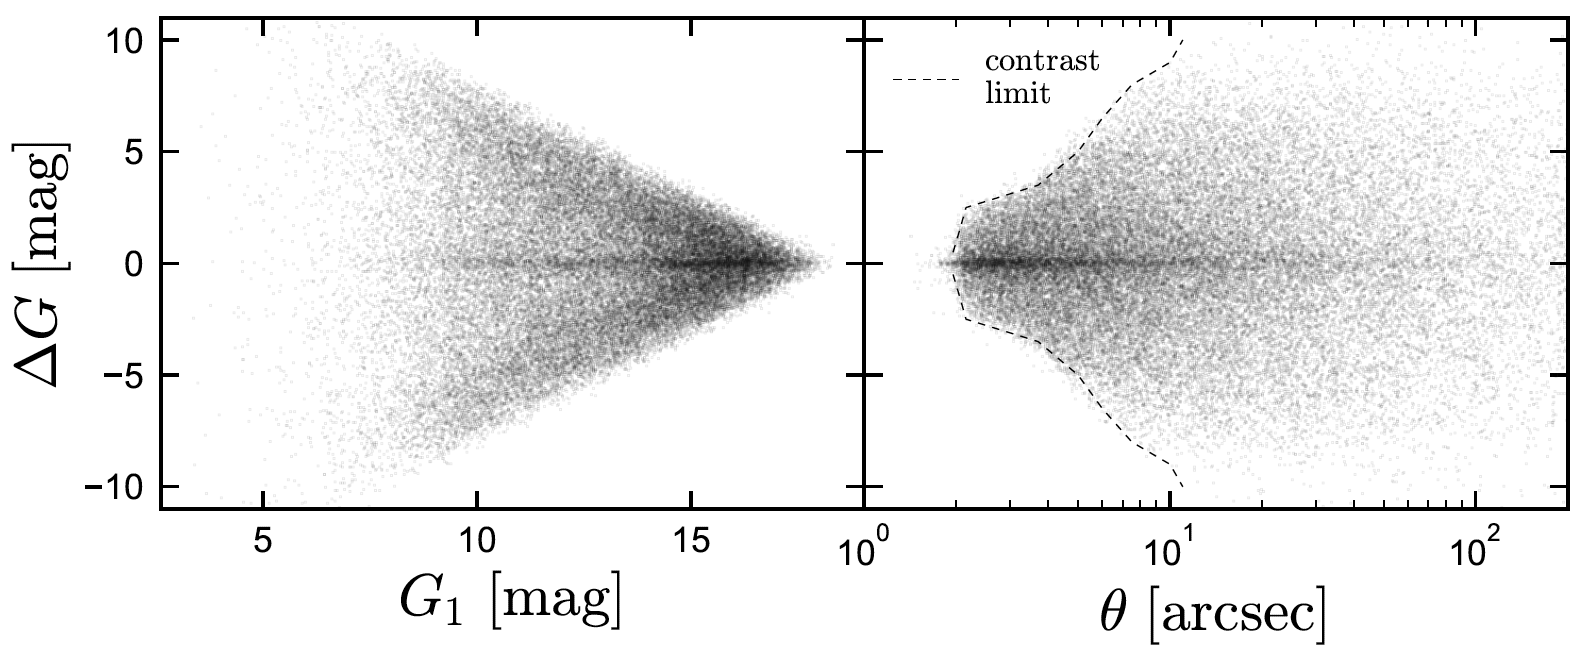
\includegraphics[width=0.7\linewidth]{img/BinarySelection_ElBadry.png}
    \caption{Illustration of the inherent complexities of the Gaia selection function (`contrast limit', right panel), when considering close pairs of sources, from \citet{ElBadry2019}, who discovered a population of twin-binaries (near-identical stars) to $\gtrsim 1000$~AU of unknown formation mechanism.
    Unsurprisingly, the minimal angular separation at which stars of a certain magnitude difference $\delta$G have both good proper motions (to be recognized as comoving) depends strongly on $\delta$G}
    \label{fig:binaries}
\end{figure}

Binaries are in this respect only the minimal case of either a star cluster or of crowded stellar fields in general. It is unsurprising that not a single publication using Gaia DR2 has appeared on one of the most interesting directions in our Galaxy, Baade's window.
In crowded field, often the catalog existence BP and RP ``magnitudes'',
which come from re-integrated slitless spectra, have a very complex dependence on position and magnitude.

\textbf{Without rigorous knowledge of $S_C(y_s)$ in the `crowded source' regime, binary science, cluster science and the central Galaxy will remain inaccessible to Gaia studies that do justice to the data's information content.}

There are added levels of complexity of determining and characterizing the selection function. Often, is of interest -- or at least tempting -- to make an extensive set of of quality flags part of a sample selection. If such cuts only eliminate a tiny subset, for reasons unrelated to the object's physical properties, this is without consequence. But if far-reaching cuts are made in quality flags such as RUWE (renormalized unit weight error) or on data uncertainties (velocity errors, fractional parallax errors) a whole new level of complexities arises. While in general it may be advisable to base sample selection on observables, not their uncertainties, the issue cannot be ignored. 
This is an area, where it may not be possible to devise (in the context of this proposal) a user-ready recipe for $S_C(y_s)$.

\textbf{Taken together, far better knowledge of the Gaia catalog selection function $S_C(y_s)$ is needed to
\begin{itemize}
    \item map our galaxy in 3D 
    \item do galaxy dynamics, constrain the distribution of dark matter and detect `empty' dark matter halos
    \item  unleash Gaia's potential for stellar astrophysics, even on aspects as elementary as estimating luminosity functions and frequencies of special objects, or learn about binary stars.
    \item start exploring what Gaia can teach us in `crowded fields', clusters and the inner galaxy.
\end{itemize}
In short, better knowledge of the Gaia catalog selection function $S_C(y_s)$ is indispensible, and not part of the DPAC deliverables.}

In the subsequent sections we lay out how to provide this.  We will focus on the 
position-magnitude aspects of the selection function, and on the selection function that arise when combining Gaia data sets with external information, spectroscopic surveys or deeper imaging surveys.


% A selection function quantifies how the objects in an astronomical catalogue were chosen from the countless asteroids, planets, stars and galaxies in the Universe. Without the selection function,
% %we can only make state
% %Without a selection function,
% it is impossible to extrapolate from \textit{statements about the objects in a catalogue} into \textit{insights in fundamental physics}. 

% The selection function is necessary in order to draw conclusions about fundamental physics from the limited and biased fraction of objects in our catalogues. Without a selection function, we could only make statements about the objects in our catalogues.

% The selection function can be calculated \By{MF}{should be calculable?} for any hypothetical object, returning one if that object would have been included in the catalogue and zero if not. The selection function can also take values between zero and one, in which case we interpret the selection function as giving the probability that the object would appear in the catalogue.

% The Gaia selection function is hard.

% Detailed motivation of the need for a selection, use a few example science cases to make the point.

% \begin{itemize}
%     \item What prominent Gaia science cases cannot (ever?) be done without a well-defined and computationally tractable
%         selection function
%         \begin{itemize}
%             \item Structural parameters of the Milky Way (disk scale length/height etc)
%             \item Dark matter sub-halo finding through gaps in streams
%             \item Binary population parameters (frequency, parameter distributions), but also stellar census (mass function of single stars)
%             \item Exoplanet population parameters (frequency, parameter distributions)
%             \item Local dark matter density
%         \end{itemize}
%     \item What is the selection function.
%         \begin{itemize}
%             \item Needs to be clearly defined and will probably require someone to work on the detailed definition and
%                 mathematical formulation (if the latter has not already been done).
%             \item How does it relate to survey completeness; do we include completeness in the definition.
%             \item Point out that multiple layers of selection may take place in any scientific investigation of Gaia or
%                 other astronomy data. The formulation/definition of the selection function should allow for layers of
%                 selection.
%             \item To keep the work manageable in this project we will only provide the `basic' Gaia selection function.
%                 Accounting for the effect of additional user-imposed selection of data will be through tools also
%                 developed in this project.
%         \end{itemize}
%     \item Impact on the rest of astrophysics
%         \begin{itemize}
%             \item The Gaia catalogue is now being used to define target selection for other surveys (e.g. 4MOST). The completeness of these derivative surveys will be defined by the completeness of Gaia.
%             \item We will implement selection functions for other surveys (e.g. APOGEE, LAMOST) in the open source software that we produce, that will enable users to, for example, calculate the odds of a star having a parallax in Gaia and a radial velocity in APOGEE.
%         \end{itemize}
% \end{itemize}

% some references
%
% Selection function work in various MW surveys.
% the Geneva Copenhagen Survey - GCS by Schönrich & Binney, 2009; Sharma et al., 2014.
% the Sloan Extension for Galactic Understanding and Exploration - SEGUE by Bovy et al., 2012; Cheng et al., 2012; Schlesinger et al., 2012.
% the APO Galactic Evolution Experiment - APOGEE by Bovy et al., 2014; Nidever et al., 2014; Anders et al., 2016.
% the Large sky Area Multi-Object fiber Spectroscopic Telescope experiment - LAMOST by Carlin et al., 2012; Yuan et al., 2015.
% the RAdial Velocity Experiment - RAVE by Sharma et al., 2011, 2014; Francis, 2013; Wojno et al., 2017.
% the Gaia-ESO Survey - GES by Stonkute et al., 2016.
% the Tycho Gaia astrometric solution - TGAS by Bovy, 2017.

% Population synthesis and dynamical models of the MW
% Besan{\c{c}}on (Robin et al., 2003), 
% TRILEGAL (Girardi et al., 2005),
% GALAXIA (Sharma et al., 2011).


\section{Relation to the work programme}
\label{sec:relation-to-work-programme}
\instructions{
Indicate the work programme topic to which your proposal relates, and explain how your proposal
addresses the specific challenge and scope of that topic, as set out in the work programme.
}

This proposal is in response to the call ``Space 2018--2020'' and is specifically focused on the topic ``Scientific Data Exploitation'' (SPACE-30-SCI-2020). The work proposed here addresses the SPACE-30-SCI-2020 challenges as follows:
\begin{itemize}
    \item Researching, developing, implementing and publicly providing a detailed Gaia survey selection function will (as motivated above) very much enhance the scientific data exploitation of a flagship European (ESA) space mission. In particular the data from the Gaia mission will have a legacy value for many decades to come. The future scientific exploitation of the Gaia legacy archive will also benefit tremendously from a readily available detailed selection function. This also holds for future astrophysics missions which rely in some way on Gaia (target selection, calibration) or are a follow-ups to Gaia.
    \item The development of the Gaia selection function will, among others, involve a comparison to or combination with data from other surveys, both ground and space based (see \secref{sec:methods} and \ref{wp:selfuncombine}). This will enhance our insights into the Gaia selection function but also provide new insights into the selection functions of the other surveys and boost the scientific exploitation of their data.
    \item The expertise built up in constructing the Gaia selection function can be transferred to other surveys and thus enhance the science exploitation of future European space missions, or even inform the design of such missions to ensure the resulting surveys have tractable selection functions.
    \item The work proposed here will lead to data products that can be integrated into the ESA Gaia archive and to open source software tools which will be made available through code hosting websites. The combination of data and code will enable the users to include in their scientific analyses the Gaia selection function as well as selection functions for Gaia combined with other surveys.
    \item The participants in this proposal represent an international collaboration with in particular the involvement of partners from the USA and Australia, both countries which are active in space exploration and space science.
\end{itemize}

\section{Concept and methodology}
\label{sec:conceptandmethods}
\subsection{(a) Concept}
\label{sec:concept}
\instructions{
    \begin{itemize}
        \item Describe and explain the overall concept underpinning the project. Describe the main
            ideas, models or assumptions involved. Identify any inter-disciplinary considerations and,
            where relevant, use of stakeholder knowledge. Where relevant, include measures taken for
            public/societal engagement on issues related to the project. Describe the positioning of the
            project e.g. where it is situated in the spectrum from ‘idea to application’, or from ‘lab to
            market’. Refer to Technology Readiness Levels where relevant. (See General Annex G of the work
            program);
        \item Describe any national or international research and innovation activities which will be
            linked with the project, especially where the outputs from these will feed into the project;
    \end{itemize}
}

The basic concept for this project is to go from the idea of having available a selection function to enhance the science exploitation of the Gaia catalogue data to a publicly available practical implementation which can be applied by scientist in the scientific exploitation of the Gaia data. This will be achieved through research and development conducted at the partner institutes. The bulk of the effort is budgeted for the European partners but essential expertise and effort will contributed by the partners in the US and Australia. The realization of the Gaia selection function requires: 
\begin{itemize}
    \item an operational (mathematical) definition of the concept of a selection function as a framework for the overall effort;
    \item a detailed understanding of the Gaia sky scanning history and the various points at which measurements or objects are lost or discarded for one reason or another;
    \item bringing the above together in a specific realization the selection function for Gaia;
    \item providing the necessary software tools and numerical data to enable scientists to incorporate the selection function in their analyses of the Gaia data (combined with other survey data).
\end{itemize}
The whole effort must be guided by developing in parallel a number of concrete and diverse science applications in order to ensure that the requirements on the selection function (level of detail, best practical implementation) are properly understood and incorporated in the data products and tools delivered through the efforts proposed here. \secrefcap{sec:methods} describes in detail how the above elements are implemented through the work packages listed in \ref{sec:work-plan}.

The stakeholders in this effort are the astronomical scientific community, which will benefit from the enhanced capability to exploit the Gaia (and other survey) data; the DPAC will profit from the detailed understanding of the selection function during the quality control of the Gaia data products and gain insights into how to improve the data processing such that the selection function is kept as simple and tractable as possible; ESA will benefit from insights into future mission design that grow out of the detailed investigations of the selection function and from the strongly enhanced legacy value of the Gaia archive combined with the tools to properly account for selection effects; Other sky survey projects which either base their target lists on the Gaia catalogue or use Gaia data as a reference for their calibrations will benefit from a detailed understanding of how their selection functions are affected by the use of Gaia data. In return the expertise of these stakeholders will benefit this project: the scientific community will be engaged through publicly available prototypes of the {\acro} tools and through community workshop at which user feedback and requirements can be captured; DPAC will play a natural role in understanding in detail all the selection effects entering the Gaia catalogue; the ESA expertise with data archiving and dissemination can be tapped for the efforts to make the selection function publicly available; the data from other sky surveys will be used in the research on the Gaia selection function proposed here.

The links to ESA and DPAC are a natural element in this proposal because of the role of the coordinator and the contact persons at the European partners within the DPAC consortium (see \secref{sec:consortium}). The links to the scientific community are established through the academic institutes where the work will take place and through participation in international workshops and conferences. Further links exist with the MW-Gaia COST action in which several of the partners on this proposal participate. This will facilitate participation in workshop and conferences organized by MW-Gaia which are natural venues for the dissemination of the knowledge and tools built within {\acro}.

\begin{figure}[t]
    \centering
    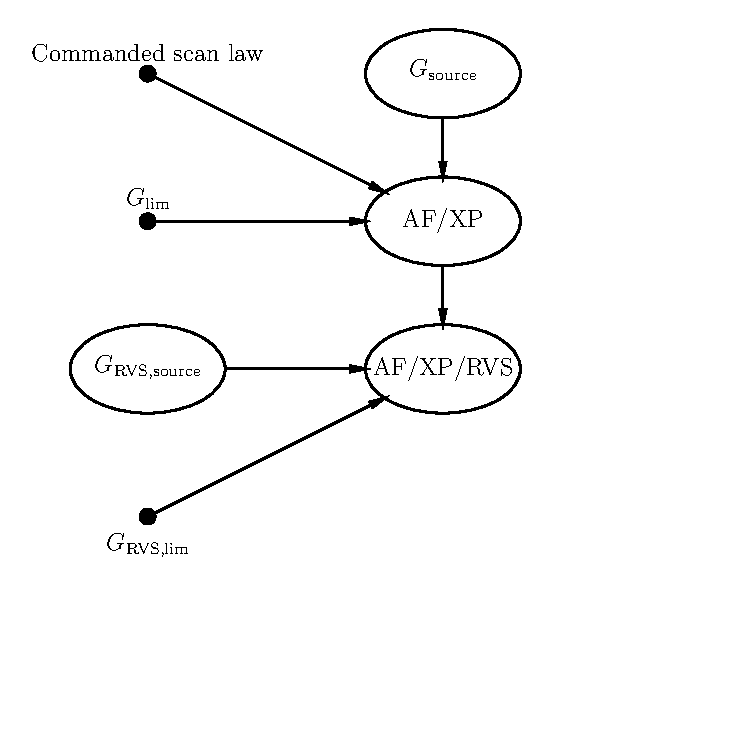
\includegraphics[height=8cm]{pgm_ideal_gsf.pdf}
    \caption{Idealized Gaia selection function. Here it is assumed that the spacecraft exactly follows the scan law as commanded from ground without any interruptions. The on-board decision on whether or not a source is observed depends only on the $G$ and $G_\mathrm{RVS}$ magnitudes of the source and the corresponding fixed survey limits. See text for a more detailed explanation.}
    \label{fig:gsf_ideal}
\end{figure}

\subsection{(b) Methodology}
\label{sec:methods}
\instructions{
    \begin{itemize}
        \item Describe and explain the overall methodology, distinguishing, as appropriate, activities
            indicated in the relevant section of the work programme, e.g. for research, demonstration,
            piloting, first market replication, etc.
    \end{itemize}
}

The Gaia selection function in an ideal world would look like the probabilistic graphical model shown in \figref{fig:gsf_ideal}. In this figure and the subsequent text the three main Gaia instruments as referred to as `AF' for Astrometric Field (collecting the astrometric data), `XP' which is short for the BP and RP photometric instruments, and RVS, the radial velocity spectrometer. The model in \figref{fig:gsf_ideal} shows that AF and XP observations of sources are collected whenever one of the Gaia telescopes scans over a source which has a magnitude $G_\mathrm{source}$ brighter than the magnitude limit $G_\mathrm{lim}$. If a source is bright enough in $G_\mathrm{RVS}$ data are also collected by the RVS instrument. The pointing of the Gaia telescopes is determined by a `scan law' which is fixed for the mission duration. The probability of a source entering the Gaia catalogue would thus be determined only by its true apparent magnitude $G_mathrm{source}$, the number of times the Gaia telescopes scanned across the source, and the uncertainty $\sigma_G$ in the on-board estimate of the source brightness. The probability that a radial velocity is listed in addition to astrometry and photometry would be determined independently by the true apparent magnitude of the source in the RVS wavelength range, $G_\mathrm{RVS,source}$, in combination with the scan law and the uncertainty $\sigma_{G_\mathrm{RVS}}$ of the on-board estimate of $G_\mathrm{RVS,source}$. The selection function for any derived data products, such as the astrophysical parameters of the sources, would be driven entirely by the basic data (astrometry, photometry, radial velocity, XP spectra, RVS spectra, or any combination thereof) used as inputs.

\begin{figure}[t]
    \centering
    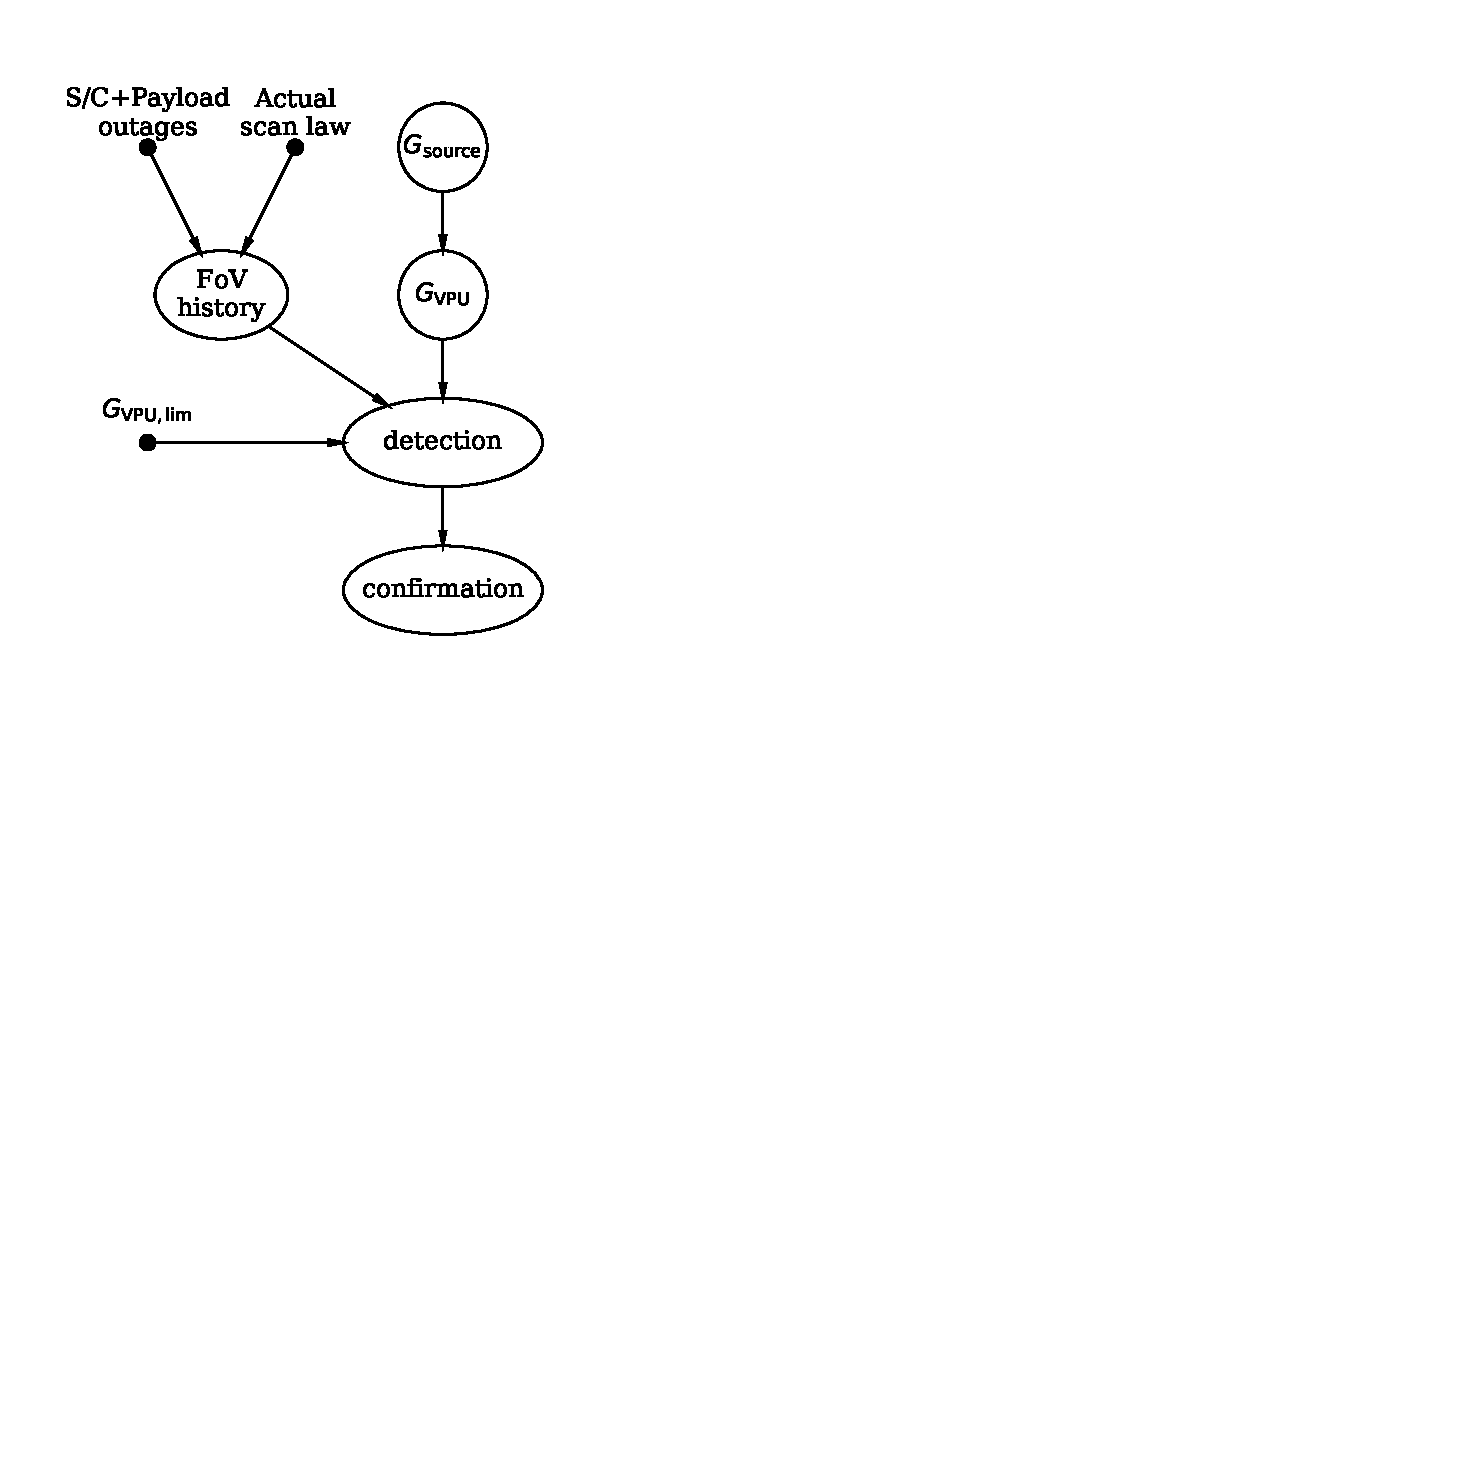
\includegraphics[width=\textwidth]{pgm_realistic_gsf.pdf}
    \caption{Simplified diagram of the actual Gaia selection function. The left hand side of the diagram provides a fairly complete picture of all the ingredients on-board the spacecraft that contribute to the selection function before the raw data is in hand on the ground. The right hand side shows in strongly simplified form how the Gaia selection function is further affected by the decision taken along the steps from the initial treatment of the raw data to the final published Gaia catalogue. See text for more detailed explanations.}
    \label{fig:gsf_realistic}
\end{figure}

In reality the Gaia survey selection function is vastly more complicated owing to the many stages in between source detection and final data product at which decisions are made on the spacecraft whether or not to make a certain observation, and in the on-ground data processing whether or not to include that observation. This is illustrated in \figref{fig:gsf_realistic}. The left hand side of the diagram shows the many decisions that are taken on-board the spacecraft which affect whether or not for a given source, passing through the field of view of one of the telescopes, measurements are actually collected.
\begin{itemize}
    \item The actual sky-scanning strategy executed by Gaia will differ from the desired one due to imperfections in the attitude control and interruptions of observations due to outages such as station keeping manoeuvres or on-board activities that require interrupting the measurement process (e.g., decontamination through heating of the payload, refocusing of the telescopes, more details can be found in \cite{2016A&A...595A...1G}).
    \item At the detection stage the brightness of the sources is estimated (with some uncertainty). This is indicated by $G_\mathrm{VPU}$ in the \figref{fig:gsf_realistic}, where VPU stands for `Video Processing Unit', essentially an on-board computer. In parallel an attempt is done to weed out spurious detections due to cosmic rays or PSF spikes, and sources are prioritized in order to deal with the limitation on the amount of sources that can be handled by the VPUs at any one time.
    \item Following confirmation that a detected source is real (through a second measurement of the source flux) astrometric and photometric data are collected, subject to further limitations in the amount of sources that can handled (indicated with 'VPU resource management' in \figref{fig:gsf_realistic}).
    \item RVS observations are collected only for sources bright enough in $G_\mathrm{RVS}$ which is estimated for bright sources through extrapolation from the on-board estimate $G_\mathrm{VPU}$ of $G_\mathrm{source}$ or through an estimate $G_\mathrm{RVS,VPU}$ from the flux in the RP spectrophotometric data. The latter introduces a source colour dependence.
    \item The data collected on-board is partly transmitted to the ground stations in real-time (during spacecraft contact periods) and is partly stored on-board for later transmission. The on-board storage limitations lead to data being deleted if it stays in the storage area too long (a consequence of limited availability of ground station time and the size of the data storage area). This happens primarily during so-called `galactic plane scans', when both Gaia telescopes are pointing at locations in the Milky Way plane on the sky. The data deletion decision is taken on the basis of a detailed priority table stored on-board. Additional data losses may occur due to lost telemetry packets (a minor contribution affecting roughly one in a million packets).
\end{itemize}

The left hand side of \figref{fig:gsf_realistic} shows a strongly simplified representation of further decisions taken along the DPAC pipelines on whether or not to process certain sources or parts of their data.
\begin{itemize}
    \item As a first step in the processing sources are classified as real or spurious, where the latter are typically caused by bright star PSF spikes or stray light features. Sources classified as spurious are `blacklisted' and subsequently not considered for processing. This classification process is imperfect.
    \item The next step is to group observations of the same source together and produce the so-called `source list'. This is a table linking a given source to all its observations. This process is redone from scratch for each data release and is subject to errors, such as observations being assigned to the wrong source, or the observations of one sources being assigned to multiple different sources. Two examples of specific challenges for the creation of the source list are crowded regions, where the source density on the sky can lead to observation to source matching uncertainties, and variable stars, where a strongly varying apparent brightness can confuse the matching process.
    \item Once the source list is created all subsequent processing steps are taken, from generating the astrometry, photometry, and radial velocity data, to the astrophysical characterization of sources, to the publication of a Gaia data release. At each step further decisions are taken on including or not sources or parts of their data. Often these decisions are explicitly or implicitly dependent on the source astrophysical parameters which will introduce further source brightness and colour dependencies into the selection function.
\end{itemize}

From the description above it is clear that the Gaia survey selection function is very complex and depending on the particular science case being addressed with Gaia data, the selection function must be known in great detail. An example is the list of binaries to be produced on the basis of Gaia data. The list will consist of various solution types (varying from mere indications of binarity to complete orbit solutions) which will be derived only for sources for which there is sufficient evidence that they are not single stars. The resulting list will thus be incomplete in a way that intricately depends on the binary star parameters, with many binaries still hiding among the sources not examined in detail in the DPAC pipeline.

The objective of this proposal is to derive a detailed description of the Gaia selection function which will be provided to and used by the scientific community. This will be done through the following tasks which map to the work packages listed in \secref{sec:work-plan} (the management task, work package \ref{wp:management}, is discussed in \secref{sec:management}).

\begin{description}
    \item[Operational definition of the Gaia survey selection function.] To guide the overall effort on the Gaia selection function it is important to precisely define what we mean by a selection function. We choose to take a probabilistic approach, thus asking the question: what is the probability of source X appearing in sub-sample Y of the Gaia catalogue? The mathematical formulation should at the top level be applicable to any astronomical survey but detailed mathematical definitions tailored to the Gaia survey may be needed. The formulation should account for the multiple layers of selection described above and allow for incomplete information on the data collection process. The formulation should also make it possible to accommodate additional user imposed selections (such as studying only sources with certain astrophysical parameters or demanding a minimum precision on the data used). A hierarchical probabilistic formulation is a natural choice but other approaches are not excluded. This task corresponds to work package \ref{wp:selfundefinition} and should be completed within the first 12 months of this project.
    \item[Specification of the Gaia selection function.] With the above mathematical formulation as the framework, this task is concerned with researching and working out in detail the description and modelling of the Gaia survey selection function (where we anticipate that some aspects cannot be described in all detail and will require simplifications or modelling). All the necessary information will be collected to describe or model in detail the elements in \figref{fig:gsf_realistic}, which will require close interactions with experts from the DPAC. An assessment will be made of the necessary level of detail to which the ingredients of the selection function must be known (in order to keep the scope of the effort realistic). The resulting description of the selection function will be hierarchical, starting from the basic selection steps and specializing to selection functions for specific subsets of the Gaia catalogue (such as, for example, the variable stars), and will allow for the inclusion of user imposed additional selection criteria. Part of this task will also be to collect data from other surveys which may aid in the understanding of the Gaia selection function. Examples are higher spatial resolution data from the Hubble Space Telescope to study selection effects in crowded regions, or photometric/spectroscopic data which can aid in the understanding of the selection effects on the distribution of source astrophysical parameters in Gaia samples. This task corresponds to work package \ref{wp:selfungaia}.
    \item[Tools to incorporate selection function in scientific analyses.] The aid the scientific community in using the Gaia selection function a set of data products and tools will be provided. The tools will implement in code the mathematical formulation and detailed description/modelling of the Gaia selection function. A means to layer user selections on top of the Gaia selection function will also be provided. The tools will be backed by the data products needed to use them such as numerical tables. These data products will be made available through, e.g., \url{https://zenodo.org/}, and in query-able form through the Gaia archive at ESA. The code underlying the tools will be open source and accessible through popular code-hosting facilities such as \url{https://github.com/}. Extensive documentation will also be provided in the form of papers in open access journals and detailed online documentation. This task corresponds to work package \ref{wp:selfunimplementation}.
    \item[Selection functions for combinations of Gaia and other surveys.] In many science applications the Gaia data will be combined with data from other surveys, often leading to the production of catalogues based on the input surveys \citep[see for example][]{2019A&A...628A..94A}. In such applications one needs to account for the combined selection function for the intersection of the surveys involved. In this task a generic method to combine survey selection functions will be researched and developed. The method will then be applied to generate selection functions for the combination of Gaia and a limited number of popular sky surveys. The tools and data products needed to combine selection functions will be made available through the channels mentioned above. The scientific community can use these to construct selection functions for other combinations of surveys. An important component of this task is making prototype versions of the tools publicly available and to bring users together in community workshop to use and test the tools. The feedback will be used to improve the prototypes. This task corresponds to work package \ref{wp:selfuncombine}.
    \item[Apply the selection function tools to selected science cases.] We believe that the best way to guide the overall efforts in this proposal and to thoroughly test the implementation of the Gaia survey selection functions, is to apply it to a number of science cases. The science cases will be developed in parallel to the selection function, both as a means to provide early tests of -- and feedback to -- the tasks above, and as a means to keep the researchers involved in this effort motivated. The results of the science applications will be published in the open access peer reviewed literature. It is very important for their future career that the post-doctoral researchers carrying out the bulk of the work will also have a publication featuring a science application to add to their CVs. This task corresponds to work package \ref{wp:scienceappl}.
\end{description}

\section{Ambition}
\label{sec:ambition}
\instructions{
    \begin{itemize}
        \item Describe the advance your proposal would provide beyond the state-of-the-art, and the
            extent the proposed work is ambitious.
        \item Describe the innovation potential (e.g. ground-breaking objectives, novel concepts and
            approaches, new products, services or business and organisational models) which the proposal
            represents. Where relevant, refer to products and services already available on the market.
            Please refer to the results of any patent search carried out.
    \end{itemize}
}

As pointed out in \secref{sec:objectives} there is currently no detailed selection function available for the Gaia survey. It is not part of the DPAC tasks or data products, and the limited attempts that have been made in the community to characterize the selection function have led mostly to ad-hoc implementations for specific science cases. In fact the vast majority of works on the Gaia data so far ignore the selection effects altogether. More generic attempts at describing the Gaia selection function have been undertaken by Boubert \& Everall\footnote{\url{https://github.com/DouglasBoubert/selectionfunctions}}, and by Rybizki, Drimmel \& Carrasco\footnote{\url{https://github.com/jan-rybizki/gdr2_completeness}}. However, these efforts only scratch the surface of the complexities of the Gaia selection function. The efforts proposed here will thus go well beyond the state of the art:
\begin{itemize}
    \item For the first time a Gaia survey selection function will be provided at the level of detail and with the tools needed to take it into account in any science application.
    \item The efforts to describe and implement the Gaia selection function will lead to a clarification and better definition of the concept of selection functions and biases. This will benefit the development of selection functions for other surveys.
    \item The availability of the selection function will enhance all the scientific analyses of the Gaia data. This will lead to a much better scientific exploitation of the Gaia data in that selection biases can be properly accounted for, while the availability of open source tools and corresponding open access data will facilitate a much better reproducibility of results.
    \item The innovations in terms of the mathematical formulation of the selection function and a usable detailed practical implementation thereof can be transferred to other sky surveys, both past and future, enhancing the quality of the scientific exploitation and their legacy value.
\end{itemize}

%%% Local Variables:
%%% mode: latex
%%% TeX-master: "proposal-main"
%%% End:
 % Section I
\chapter{Impact}
\label{cha:impact}


\section{Expected impacts} 
\label{sec:expected-impact}
\instructions{
\begin{itemize}
    \item Describe how your project will contribute to:
    \begin{itemize}
        \item each of the expected impacts mentioned in the work programme, under the relevant topic;
        \item any substantial impacts not mentioned in the work programme, that would enhance innovation capacity; create new market opportunities, strengthen competitiveness and growth of companies, address issues related to climate change or the environment, or  bring other important benefits for society
    \end{itemize}
    \item Describe any barriers/obstacles, and any framework conditions (such as regulation, standards, public acceptance, workforce considerations, financing of follow-up steps, cooperation of other links in the value chain), that may determine whether and to what extent the expected impacts will be achieved. (This should not include any risk factors concerning implementation, as covered in section 3.2.)
\end{itemize}
}

We expect the following impacts directly related to the work programme:
\begin{itemize}
    \item The availability of a detailed Gaia selection function coupled with the data and tools to use it will enhance the quality and reproducibility the scientific exploitation of data from this flagship European space mission. Thus great value is added to the existing European efforts dedicated to the data processing for the Gaia mission as well as to the efforts to produce the publicly available Gaia data releases.
    \item A readily available Gaia selection function will enable addressing science cases that are currently hampered by the lack of a detailed description of Gaia survey selection biases. This will translate in an increase in the number of scientific publications based on European space missions.
    \item We will make data products and tool available for a much more advanced analysis of Gaia and other survey data than is currently possible.
    \item Although the participants on this proposal have all worked together in various constellations in the past on different topics, this is the first time that this group of experts willing to invest time in the details of the Gaia selection function will work closely together, this enhancing an existing loose collaboration and broadening the expertise of all involved.
    \item The expertise on the Gaia selection function will be transferred to DPAC. This will facilitate turning the selection function into a standard DPAC data product for the community. In addition a detailed selection function allows for a more careful validation of the DPAC data products. For example, features in the population statistics of sub-samples of the Gaia data can then be correctly attributed to a selection bias or a problem in the data processing. The result will be better quality control before a Gaia data release.
    \item The expertise gained in this project can be transferred to other surveys. This is already partly planned in this proposal through work package \ref{wp:selfuncombine} on combined selection functions. However we expect that beyond that other survey teams will seek out the expertise developed in this project pick up the method and tools we make available. This will enhance both European and international activities. Examples of future European projects that stand to benefit are the 4MOST and WEAVE spectroscopic surveys and the Euclid and Plato space missions. Examples of international projects that would benefit are future surveys such as LSST (US) as well as existing surveys such as GALAH (Australia) which rely heavily on complementary Gaia data.
\end{itemize}

On a broader societal level the impact will be through the expertise built up with understanding in detail how the interpretation of large amounts of collected data is affected by selection biases and how this limitation can be addressed through a proper description of the way the data was collected. This will be of benefit to any data science application and we expect that some of the researchers funded through this proposal might opt for a future career in European companies of which the business contains a large data science component.

Other than the normal risks associated with scientific research we do not foresee any barriers to achieving the impacts above. The project does of course have some risk factors as listed in \secref{sec:management}.

\section{Measures to maximize impact} 
\label{sec:maximize-impact}

\subsection{a) Dissemination and exploitation of results}
\label{sec:dissemination-exploitation}
\instructions{
\begin{itemize}
    \item Provide a draft `plan for the dissemination and exploitation of the project's results'. Please note that such a draft plan is an admissibility condition, unless the work programme topic explicitly states that such a plan is not required.\\
    Show how the proposed measures will help to achieve the expected impact of the project.\\
    The plan, should be proportionate to the scale of the project, and should contain measures to be implemented both during and after the end of the project. For innovation actions, in particular, please describe a credible path to deliver these innovations to the market.
    \item Include a business plan where relevant.
    \item As relevant, include information on how the participants will manage the research data generated and/or collected during the project, in particular addressing the following issues:
    \begin{itemize}
        \item What types of data will the project generate/collect? o What standards will be used? 
        \item How will this data be exploited and/or shared/made accessible for verification and re-use? If data cannot be made available, explain why.
        \item How will this data be curated and preserved? 
        \item How will the costs for data curation and preservation be covered?
    \end{itemize}
    \item Outline the strategy for knowledge management and protection. Include measures to provide open access (free on-line access, as the `green' or `gold' model) to peer-reviewed scientific publications which might result from the project.
\end{itemize}
}

\subsubsection{Draft plan for the dissemination and exploitation of the project's results}

The area in which we expect to make the largest impact is the scientific exploitation of results from the Gaia mission and other surveys. Correspondingly our dissemination efforts will be aimed at scientists using astronomical survey data and we will primarily use the standard academic channels:
\begin{itemize}
    \item Presentation, description and documentation of our results through scientific publications in peer-reviewed journals. We will make use of open access journals (`gold' open access) and we will always make our publications available through \url{https://arxiv.org} (`green' open access).
    \item Our results will be presented and promoted at scientific meetings where we aim to reach a diverse audience through the variety of science applications addressed as part of our efforts.
    \item We will organize a community workshop in which the Gaia selection function experts will offer training to interested scientists in the use of our data products and tools (deliverable \ref{dev:wp1closing}). Our results from the science applications in work package \ref{wp:scienceappl} will serve as excellent worked examples.
    \item We will discuss with colleagues providing courses in data analysis and statistics to science students how our methods and tools may be used in such courses. We will provide support to adapt our tools to the needs of the course instructors.
\end{itemize}

This project will collect the data needed to understand the Gaia selection function, such as the details of the actual scan law used or of the spacecraft operation interruptions. These data will be part of the tools needed to use the Gaia selection function and thus will be stored in a form suitable for computer use or for storage in a database.
\begin{itemize}
    \item All data generated/collected in this project will be made available publicly. This will be done through the ESA Gaia archives and any other astronomical data centres interested in hosting these data. In addition the data will be deposited with \url{https://zenodo.org}.
    \item The source code for the computer tools will be made available publicly through well known open access source code repositories such as \url{http://github.com} or through code hosting services available at the institutes participating in this proposal.
    \item A website will be setup (hosted by Leiden University) which will serve as entry point to the data, tools, and documentation generated in this project. To enhance visibility cross-links will be made with, for example, ESA websites related to Gaia.
\end{itemize}

The Gaia mission operations will end at the latest around end 2024 and the data processing will continue for a number years thereafter before the final (legacy) Gaia archive version can be released. This is beyond the lifetime of the project proposed here and we thus intend to transfer the expertise on the selection function to the DPAC aiming to make the selection function a data product provided by DPAC. This is most naturally done through the ESA archive and will include documentation. Hence a long term curation of the corresponding data is foreseen as part of the Gaia legacy archive maintained by ESA. Note that the maintenance of this archive is mandatory as the Gaia data is expected to set the standard in astrometric data for decades to come. \memo{Say something on long term code preservation, perhaps make the tools part of a larger ecosystem like Astropy?}

\subsection{b) Communication activities}
\label{sec:communication-activities}
\instructions{
\begin{itemize}
    \item Describe the proposed communication measures for promoting the project and its findings during the period of the grant. Measures should be proportionate to the scale of the project, with clear objectives.  They should be tailored to the needs of different target audiences, including groups beyond the project's own community.
\end{itemize}
}

As mentioned above the community explicitly targeted by this proposal, professional astronomers, will be reached through the well known academic outreach channels: scientific publications, presentations at scientific conferences, and open access to the data and tools resulting from this project. In addition we plan to engage the general public through media releases of the results from application of the Gaia selection function to specific science cases, highlighting how the work on the selection function enables much better interpretation of, for example, binary star and exoplanet population statistics. This will also be used as a hook to explain how a science like astronomy can enhance data analysis capabilities for society at large. \memo{Like what specifically?}
 % Section II
\chapter{Implementation}
\label{cha:implementation}

\section{Work plan --- Work packages, deliverables}
\label{sec:work-plan}

\subsection{Overall structure}
\label{sec:wpstructure}

The overall approach to the work plan is to have the research and development of the selection function progress in parallel with the implementation thereof. We made this choice because of the complexities of the selection function and its realization in the form of tools and auxiliary data, and because of the relatively short duration of the project. The work flow we foresee for {\acro} is shown in \figref{fig:workflow}. It is an iterative workflow in which the findings in each of work packages \ref{wp:selfungaia}--\ref{wp:scienceappl} will inform the others. For example the research on the selection function will lead to requirements on the implementation, while at the same time the conversion of research ideas into practical tools will lead to the questioning and revision of those same ideas. At several points during the project the results will be combined into prototype implementations of the selection function tools. These will be tested both internally to the project and through the public availability of one prototype implementation. The results from the tests will feed into the next round of research, development, and implementation. The scientific nature of much of the work conducted in {\acro} will very much benefit from an iterative approach. Close coordination between the work packages will of course be essential and this is foreseen in the management structure.

\begin{figure}
    \centering
    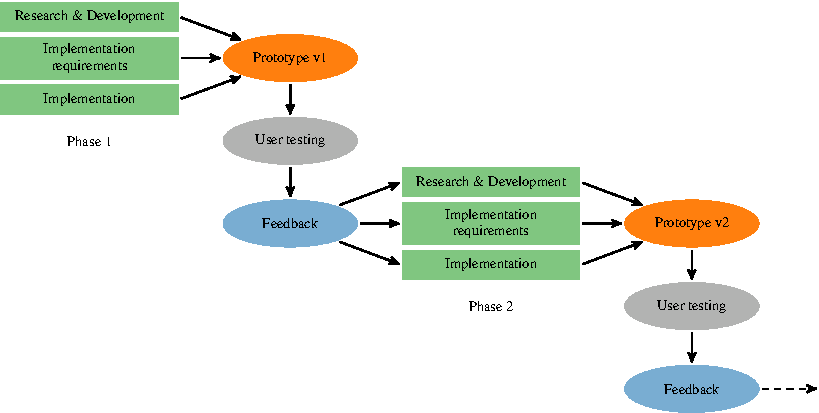
\includegraphics[width=\linewidth]{workflow.pdf}
    \caption{Iterative workflow for CoG.}
    \label{fig:workflow}
\end{figure}

\begin{figure}[ht!]
    \centering
    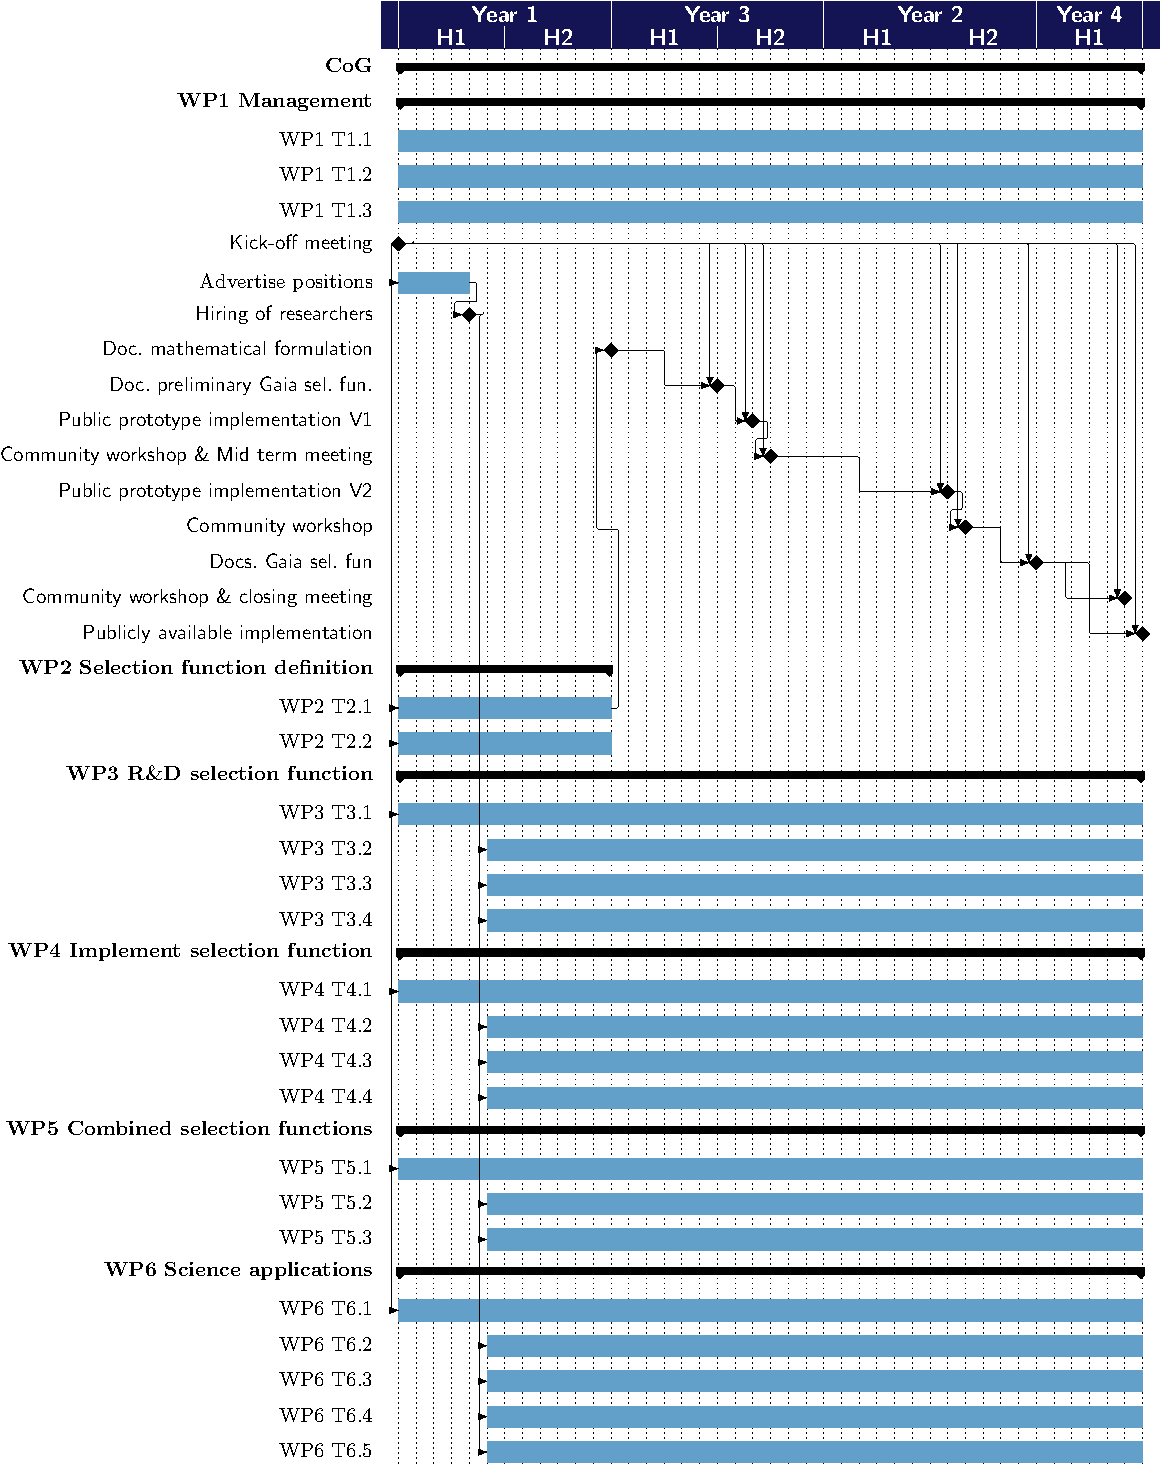
\includegraphics[width=\linewidth]{cog-gantt.pdf}
    \caption{Gantt chart for the {\acro} project.}
    \label{fig:gantt}
\end{figure}

\subsection{Timing of the work packages}
\label{sec:wptiming}

The overall work plan is structured as follows:
\begin{itemize}
    \item The first 6 months will be used to recruit the researchers to be funded from this proposal and to carry out the tasks in work package \ref{wp:selfundefinition}. Having a mathematical framework for the selection function in place early on in the project is important for guiding the research and the implementation phases.
    \item During the next three years of the project the efforts in work packages \ref{wp:selfungaia} to \ref{wp:scienceappl} will happen mostly in parallel for the reasons outlined above. The iterative approach outline in \secref{sec:wpstructure} will be used in this phase.
 \end{itemize}

\makewplist

%\subsection{Work package description}
%\label{sec:wps}

\tablecaption{Description of work packages}
\begin{supertabular}{p{\textwidth}}
    \omit \tabularnewline
\end{supertabular}
%%%%%%%%%%%%%%%%%%%%%%%%%%%%%%
%  Work Package Description  %
%%%%%%%%%%%%%%%%%%%%%%%%%%%%%%

\begin{workpackage}{Management}
  \label{wp:management} %change and use appropriate description

  %%%%%%%%%%%%%%%%%% TOP TABLE %%%%%%%%%%%%%%%%%%%%%%%%%%%%%
  % Data for the top table
  \wpstart{1} %Starting Month
  \wpend{\duration} %End Month
  \wptype{MGT} %RTD, DEM, MGT, or OTHER
  \wplead{ULEI}

  % Person Months per participant (required, max 7, * for leader)  
  % syntax: \personmonths{Participant number}{value}    (not wp leader)
  %     or  \personmonths{Participant short name}{value} (not wp leader)
  %         \personmonths*{Participant number}{value}    (wp leader)
  % for example:
  \personmonths*{ULEI}{8}
  \personmonths{MPG}{2}
  \personmonths{INAF}{2}
  \personmonths{UCAM}{2}
  \personmonths{NYU}{1}
  \personmonths{MONA}{1}
  % etc.

  \makewptable % Work package summary table

  % Work Package Objectives
  \begin{wpobjectives}
    This package provides the overall scientific coordination and administrative management of \acro\ as described in \secref{sec:management}.
  \end{wpobjectives}

  % Work Package Description
  \begin{wpdescription}
    % Divide work package into multiple tasks.
    % Use \wptask command
    % syntax: \wptask{leader}{contributors}{start-m}{end-m}{title}{description}   

    This work package includes the administrative tasks to fulfil the EC requirements and rules as
    well as the global administrative and coordination tasks inside the consortium, including financial
    management, intellectual property management and project documentation. It also includes the
    coordination with institutions and bodies relevant for the development of the Gaia archive like
    ESA, DPAC and MW-Gaia, as well as the representation of {\acro} in meetings or committees
    related to this coordination.

    \wptask{ULEI}{ULEI}{1}{\duration}{Overall coordination}{
      \label{task:wp1coordinator}
      Overall coordination and administrative management as described above (12 person-months). 
    }
    \wptask{ULEI}{MPG, INAF, UCAM}{1}{\duration}{Scientific coordination}{
      \label{task:wp1others}
      Scientific coordination by the four main partners through the {\acro} Executive Board. As stated in \secref{sec:management}, the partners NYU and MONA will have a standing invitation to meetings of the Executive Board in order to keep communications efficient.
    }    
  \end{wpdescription}
  
  % Work Package Deliverable
  \begin{wpdeliverables}
    % Data for the deliverables and milestones  tables
    % syntax: \deliverable[delivery date]{nature}{dissemination
    % level}{description} 
    %
    % nature: R = Report, DEM = Demonstrator, DEC = Websites, media, etc, OTHER = Other
    % dissemination level: PU = Public, CO = Confidential, CI = CLassified.
    % 
    % \wpdeliverable[date]{R}{PU}{A report on \ldots}

    The deliverables of this work package are the final report for the EC, the consortium agreement
    (\secref{sec:cons_agreement}), the semestral reports for the external advisory board (\secref{sec:mgtdetails}) and the organisation
    of the {\acro} plenary meetings (\secref{sec:procedures}).

    \wpdeliverable[1]{ULEI}{OTHER}{PU}{Kick-off meeting (plenary)}\label{dev:wp1kickoff}
    \wpdeliverable[2]{ULEI}{R}{PU}{Consortium agreement}\label{dev:wp1consortium_agreement}
    \wpdeliverable[6]{ULEI}{R}{PU}{Data management plan}\label{dev:wp1datamanagement}
    \wpdeliverable[6]{ULEI}{R}{PU}{Semestral report 1}\label{dev:wp1sem1}
    \wpdeliverable[12]{ULEI}{R}{PU}{Semestral report 2}\label{dev:wp1sem2}
    \wpdeliverable[18]{ULEI}{R}{PU}{Semestral report 3}\label{dev:wp1sem3}
    \wpdeliverable[21]{ULEI}{OTHER}{PU}{Mid-term meeting (plenary)}\label{dev:wp1midtterm}
    \wpdeliverable[24]{ULEI}{R}{PU}{Semestral report 4}\label{dev:wp1sem4}
    \wpdeliverable[30]{ULEI}{R}{PU}{Semestral report 5}\label{dev:wp1sem5}
    \wpdeliverable[36]{ULEI}{R}{PU}{Semestral report 6}\label{dev:wp1sem6}
    \wpdeliverable[41]{ULEI}{OTHER}{PU}{Community workshop and closing meeting}\label{dev:wp1closing}
    \wpdeliverable[\duration]{ULEI}{R}{PU}{Final report to the EC}\label{dev:wp1finalreport}
  \end{wpdeliverables}

\end{workpackage}


%%% Local Variables:
%%% mode: latex
%%% TeX-master: "proposal-main"
%%% End:

\begin{workpackage}{Definition of the selection function}
  \label{wp:selfundefinition}
  \wpstart{1} %Starting Month
  \wpend{12} %End Month
  \wptype{RTD} %RTD, DEM, MGT, or OTHER
  \wplead{MPG}
  \personmonths{ULEI}{1}
  \personmonths*{MPG}{2}
  \personmonths{INAF}{1}
  \personmonths{UCAM}{1}
  \personmonths{NYU}{1}
  \personmonths{MONA}{1}
  
  \makewptable % Work package summary table

  % Work Package Objectives
  \begin{wpobjectives}
    This objective of this work package is to research and implement a precise mathematical formulation of the concept of a survey selection function. The results will be written up as a scientific paper (to be published in the peer-reviewed literature) that will guide the rest of the work to be done within {\acro}.  The mathematical formulation of the selection function will account for the following aspects:
    \begin{itemize}
        \item Applicability to arbitrary astronomical sky surveys.
        \item The combined selection function of multiple surveys can be described within the same formalism.
        \item Accommodate multiple selection layers (e.g., the selection function intrinsic to a survey combined with additional selections imposed by the user of the data).
        \item Unknowable aspects of the selection function should be accounted for (e.g., it is not guaranteed that all sources of data loss along the detection-telemetry-processing chain for Gaia can be traced). \memo{Formulate this more precisely and in a way that makes clear this aspect can be addressed.}
        \item ...
    \end{itemize}
  \end{wpobjectives}

  % Work Package Description
  \begin{wpdescription}
    % Divide work package into multiple tasks.
    % Use \wptask command
    % syntax: \wptask{leader}{contributors}{start-m}{end-m}{title}{description}   

    \wptask{MPG}{MPG}{1}{12}{Scientific coordination}{
      \label{task:wp2coordination}
      Scientific coordination of the work on defining the selection function and coordination of writing the paper corresponding to deliverable \ref{dev:wp2document}.
    }
    \wptask{MPG}{All other}{1}{12}{R\&D formulation selection function}{
      \label{task:wp2rtd}
      Research and implement the mathematical formulation of survey selection functions.
    }

    \paragraph{Role of partners}
    \begin{description}
      \item[MPG] will lead Task~\ref{task:wp2coordination}.
      \item[ULEI, INAF, UCAM, NYU, MONA] will contribute to the research and implementation of the survey selection function mathematical formulation and will contribute to writing the paper corresponding to deliverable \ref{dev:wp2document}.
    \end{description}
  \end{wpdescription}

  % Work Package Deliverable
  \begin{wpdeliverables}
    % \wpdeliverable[date]{R}{PU}{A report on \ldots}
    \wpdeliverable[12]{MPG}{R}{PU}{Document on the mathematical formulation of survey selection functions (to be submitted to peer-reviewed journal).}\label{dev:wp2document}
  \end{wpdeliverables}

\end{workpackage}


%%% Local Variables:
%%% mode: latex
%%% TeX-master: "proposal-main"
%%% End:

\begin{workpackage}{Research and develop the Gaia selection function}
  \label{wp:selfungaia}
  \wpstart{7} %Starting Month
  \wpend{\duration} %End Month
  \wptype{RTD} %RTD, DEM, MGT, or OTHER
  \wplead{UCAM}
  \personmonths{ULEI}{2}
  \personmonths{MPIA}{6}
  \personmonths{INAF}{10}
  \personmonths*{UCAM}{23}
  \personmonths{NYU}{0}
  \personmonths{MONA}{0}
  
  \makewptable % Work package summary table

  % Work Package Objectives
  \begin{wpobjectives}
    The objective of this work package is to research and develop in detail the description and modelling of the Gaia survey selection function.
    \begin{enumerate}
      \item Develop the overall survey selection function and using that as a starting point create more specialized selection functions, focusing for example the Gaia astrometric, photometric, and spectroscopic surveys and combinations thereof. In addition a selection function for specific subsets of the Gaia survey will be developed, such as binary stars and exoplanets, variable stars, solar system objects, extragalactic sources. It will be essential here to agree to the scope of the work early on, where the development of further specialized Gaia selection function is left to the community who can make use of the tools developed in this work package. 
      \item Investigate to what extent detailed information is needed on the Gaia pointing history, its on-board detection algorithm, and the data losses introduced along the various steps from on-board measurement to the final data products. Can the selection function be reverse engineered from publicly available information?
      \item Interface with DPAC to gain a deeper understanding of the many ingredients of the Gaia selection function, in particular of aspects where public information is not (yet) available. \memo{This should be formulated more clearly.}
    \end{enumerate}
  \end{wpobjectives}

  % Work Package Description
  \begin{wpdescription}
    % Divide work package into multiple tasks.
    % Use \wptask command
    % syntax: \wptask{leader}{contributors}{start-m}{end-m}{title}{description}   

    \wptask{UCAM}{UCAM}{7}{\duration}{Scientific coordination}{
      \label{task:wp3coordination}
       Scientific coordination of the research and development of the selection function and coordination of writing the paper corresponding to deliverable \ref{dev:wp3GSFfinal}.
    }
    \wptask{UCAM}{All other}{7}{\duration}{R\&D top level selection functions}{
      \label{task:wp3toplevelGSF}
      Research and development of the top-level Gaia selection function which will describe the probability that a source enters the Gaia astrometric, photometric or radial velocity surveys, and combinations thereof.
    }    
    \wptask{MPIA}{All other}{7}{\duration}{R\&D spectroscopic selection functions}{
      \label{task:wp3spectroscopicGSF}
      Research and development of the Gaia spectroscopic selection function. This refers to the probability that a BP/RP and/or and RVS spectrum was measured for a source in the Gaia survey.
    }
    \wptask{INAF}{All other}{7}{\duration}{R\&D specialized selection functions}{
      \label{task:wp3specializedGSF}
      Research and develop the methods needed to create selection functions for specific subsets of the Gaia survey, such as binary stars or extragalactic objects. Apply this to example cases.
    }

    \paragraph{Role of partners}
    \begin{description}
      \item[UCAM] will lead Tasks~\ref{task:wp3coordination} and \ref{task:wp3toplevelGSF}.
      \item[MPIA] will lead Task~\ref{task:wp3toplevelGSF}.
      \item[INAF] will lead Task~\ref{task:wp3specializedGSF}
      \item[All partners] will contribute to the research and development of the Gaia selection functions. 
    \end{description}
  \end{wpdescription}

  % Work Package Deliverable
  \begin{wpdeliverables}
    % \wpdeliverable[date]{R}{PU}{A report on \ldots}
    \wpdeliverable[18]{UCAM}{R}{PU}{Documentation of preliminary top level Gaia selection functions.}\label{dev:wp3version1selfun}
    \wpdeliverable[36]{UCAM}{R}{PU}{Documentation of the Gaia selections functions (also to be submitted to as papers to a peer-reviewed journal)}\label{dev:wp3GSFfinal}
    \memo{Add further deliverables? Such as intermediate reports for each of the tasks above?}
  \end{wpdeliverables}

\end{workpackage}


%%% Local Variables:
%%% mode: latex
%%% TeX-master: "proposal-main"
%%% End:

\begin{workpackage}{Practical implementation and dissemination of the Gaia selection function}
  \label{wp:selfunimplementation}
  \wpstart{7} %Starting Month
  \wpend{\duration} %End Month
  \wptype{RTD} %RTD, DEM, MGT, or OTHER
  \wplead{ULEI}
  \personmonths*{ULEI}{23}
  \personmonths{MPG}{6}
  \personmonths{INAF}{2}
  \personmonths{UCAM}{2}
  \personmonths{NYU}{0}
  \personmonths{MONA}{0}
 
  \makewptable % Work package summary table

  % Work Package Objectives
  \begin{wpobjectives}
    This work package provides the practical implementation of the Gaia selection functions in terms of data and associated source code. Dissemination of these results through the ESA Gaia archive and code hosting web-sites is also part of this work package. The detailed objectives are:
    \begin{enumerate}
      \item Implement the selection function as defined and developed in detail in work packages \ref{wp:selfundefinition} and \ref{wp:selfungaia} in the form of open source code and associated numerical data (in the form of tables or any other convenient format).
      \item Implement a tool that allows for layering user defined selections on the Gaia archive data on top of the survey selection functions.
      \item Provide implementations of a number of combined selection functions for intersections of Gaia and selected other surveys.
      \item Identify code hosting options and make the Gaia selection function source code available publicly.
      \item Agree with ESA/DPAC on the hosting of the numerical data associated with the Gaia selection function in the ESA archive ecosystem.
    \end{enumerate}
  \end{wpobjectives}

  % Work Package Description
  \begin{wpdescription}
    % Divide work package into multiple tasks.
    % Use \wptask command
    % syntax: \wptask{leader}{contributors}{start-m}{end-m}{title}{description}
    \wptask{ULEI}{ULEI}{1}{\duration}{Scientific coordination}{
      \label{task:wp4coordination}
      Scientific coordination of the implementation and dissemination of the Gaia survey selection function. This includes setting up the code hosting and interfacing with ESA/DPAC on hosting the numerical data for the selection function in the Gaia archive.
    }
    \wptask{ULEI}{All other}{7}{\duration}{Implementation}{
      \label{task:wp4implement}
      Implement the Gaia selection functions in terms of open source software tools and associated numerical data. Test the implementation through applications to science cases. Port the implementation to the relevant code hosting site and transfer the numerical data to the ESA Gaia archive.
    }    
    \wptask{MPG}{All other}{7}{\duration}{Implementation of tools to include user selections}{
      \label{task:wp4layers}
      Develop and implement tools to chain together the Gaia survey selection function with additional user imposed selection on the Gaia archive data. The tools should produce an overall effective selection function for the user-selected sample.
    }
    \wptask{INAF}{All other}{7}{\duration}{Implementation of tools for combined selection functions}{
      \label{task:wp4combine}
      Implement the selection functions for combinations of Gaia and other surveys based on the methodology developed in work package \ref{wp:selfuncombine}.
    }

    \paragraph{Role of partners}
    \begin{description}
      \item[ULEI] will lead Task~\ref{task:wp4coordination}.
      \item[MPG] will lead Task~\ref{task:wp4layers}.
      \item[INAF] will lead Task~\ref{task:wp4combine}.
      \item[All partners] will contribute to the implementation and testing of the tools developed in this work package. In particular the science applications pursued by the partners will constitute a strong test of the Gaia selection function implementation.
    \end{description}
  \end{wpdescription}

  % Work Package Deliverable
  \begin{wpdeliverables}
    % \wpdeliverable[date]{R}{PU}{A report on \ldots}
    \wpdeliverable[24]{ULEI}{DEM}{PU}{Prototype of open source and open data implementation of Gaia selection function.}\label{dev:wp4prototype}
    \wpdeliverable[\duration]{ULEI}{DEC}{PU}{Open source and open data implementation of Gaia selection function.}
    \memo{Probably need a few more deliverables as concrete checks on progress.}
  \end{wpdeliverables}

\end{workpackage}


%%% Local Variables:
%%% mode: latex
%%% TeX-master: "proposal-main"
%%% End:

\begin{workpackage}{Selection function for combinations of Gaia and other surveys}
  \label{wp:selfuncombine}
  \wpstart{7} %Starting Month
  \wpend{\duration} %End Month
  \wptype{RTD} %RTD, DEM, MGT, or OTHER
  \wplead{MPIA}
  \personmonths{ULEI}{2}
  \personmonths*{MPIA}{15}
  \personmonths{INAF}{12}
  \personmonths{UCAM}{2}
  \personmonths{NYU}{0}
  \personmonths{MONA}{0}

  \makewptable % Work package summary table

  % Work Package Objectives
  \begin{wpobjectives}
    The objective of this work package is to research and develop methods to derive selection functions for the combination of Gaia and other large sky surveys. A concrete implementation for a few cases will be implemented in work package \ref{wp:selfunimplementation}. The detailed objectives are
    \begin{enumerate}
      \item Research and develop a generic method for constructing selection functions for combinations of surveys.
      \item Apply this method to a few concrete cases of the combination of Gaia with another survey.
    \end{enumerate}
  \end{wpobjectives}

  % Work Package Description
  \begin{wpdescription}
    % Divide work package into multiple tasks.
    % Use \wptask command
    % syntax: \wptask{leader}{contributors}{start-m}{end-m}{title}{description}   
    \wptask{MPIA}{All other}{7}{\duration}{Scientific coordination.}{
      \label{task:wp5coordination}
      Scientific coordination of the research and development of the combined selection function and coordination of writing the paper corresponding to deliverable \ref{dev:wp5finalreport}.
    }
    \wptask{MPIA}{All other}{7}{\duration}{Generic combination method.}{
      \label{task:wp5method}
      Research and develop a generic method for constructing selection functions for combinations of surveys.
    }
    \wptask{MPIA}{All other}{7}{\duration}{Example combined selection functions.}{
      \label{task:wp5examples}
      For a few selected examples construct the selection function for the combination of Gaia and another survey, using the method developed in task~\ref{task:wp5method}.
    }    

    \paragraph{Role of partners}
    \begin{description}
      \item[MPIA] will lead Tasks~\ref{task:wp5coordination}, \ref{task:wp5method}, and \ref{task:wp5examples}.
      \item[All other partners] will contribute to tasks \ref{task:wp5method} and \ref{task:wp5examples}.
    \end{description}
  \end{wpdescription}

  % Work Package Deliverable
  \begin{wpdeliverables}
    % \wpdeliverable[date]{R}{PU}{A report on \ldots}
    \wpdeliverable[\duration]{MPIA}{R}{PU}{Report documenting the methods to construct combined selection functions (also to be submitted to peer-reviewed journal).}\label{dev:wp5finalreport}
  \end{wpdeliverables}

\end{workpackage}


%%% Local Variables:
%%% mode: latex
%%% TeX-master: "proposal-main"
%%% End:

\begin{workpackage}{Science applications}
  \label{wp:scienceappl}
  \wpstart{7} %Starting Month
  \wpend{\duration} %End Month
  \wptype{RTD} %RTD, DEM, MGT, or OTHER
  \wplead{INAF}
  \personmonths{ULEI}{13}
  \personmonths{MPG}{13}
  \personmonths*{INAF}{15}
  \personmonths{UCAM}{13}
  \personmonths{NYU}{12}
  \personmonths{MONA}{0}

  \makewptable % Work package summary table

  % Work Package Objectives
  \begin{wpobjectives}
    The objective of this work package is to apply the Gaia selection function to four science cases. This serves to test the Gaia selection function implementation, to provide the community with worked examples of how to use the Gaia selection function, and to motivate the researchers involved in CoG and ensure that they have a scientific publication to enhance their prospects for future jobs in academia. The four science cases are:
    \begin{enumerate}
      \item Science application A. Provide a brief motivation and expected results.
      \item Science application B\ldots
      \item Science application C\ldots
      \item Science application D\ldots
    \end{enumerate}
    \memo{These are still open. Suggestions and corresponding text welcome.}
  \end{wpobjectives}

  % Work Package Description
  \begin{wpdescription}
    % Divide work package into multiple tasks.
    % Use \wptask command
    % syntax: \wptask{leader}{contributors}{start-m}{end-m}{title}{description}   
    \wptask{INAF}{All other}{7}{\duration}{Scientific coordination.}{
      \label{task:wp6coordination}
      Coordination of the efforts on the science applications of the Gaia selection function. \memo{Say a bit more about why this is needed.}
    }
    \wptask{ULEI}{All other}{7}{\duration}{Science application A.}{
      \label{task:wp6sciA}
      Carry out the research related to science application A and write a paper for a peer-reviewed journal.
    }
    \wptask{MPG}{All other}{7}{\duration}{Science application B.}{
      \label{task:wp6sciB}
      Carry out the research related to science application B and write a paper for a peer-reviewed journal.
    }
    \wptask{INAF}{All other}{7}{\duration}{Science application C.}{
      \label{task:wp6sciC}
      Carry out the research related to science application C and write a paper for a peer-reviewed journal.
    }
    \wptask{UCAM}{All other}{7}{\duration}{Science application C.}{
      \label{task:wp6sciD}
      Carry out the research related to science application C and write a paper for a peer-reviewed journal.
    }

    \paragraph{Role of partners}
    \begin{description}
      \item[ULEI] will lead Task~\ref{task:wp6sciA}.
      \item[MPG] will lead Task~\ref{task:wp6sciB}.
      \item[INAF] will lead Task~\ref{task:wp6sciC}.
      \item[UCAM] will lead Task~\ref{task:wp6sciD}.
      \item[All other partners] will contribute to tasks \ref{task:wp6sciA}--\ref{task:wp6sciD}.
    \end{description}
  \end{wpdescription}

  % Work Package Deliverable
  \begin{wpdeliverables}
    % \wpdeliverable[date]{Participant}{R}{PU}{A report on \ldots}
    \memo{Not sure we should put deliverables here.}
  \end{wpdeliverables}

\end{workpackage}


%%% Local Variables:
%%% mode: latex
%%% TeX-master: "proposal-main"
%%% End:


\makedeliverablelist

\subsection{Dependencies}
\label{sec:dependencies}

\figrefcap{fig:dependencies} shows the dependencies between the various work packages in \acro. The arrows indicate a ‘depends on’ relationship. For example WP\ref{wp:selfuncombine} depends on WP\ref{wp:selfungaia} for the details of the Gaia selection function in order to produce combined selection functions. The reverse dependency shows that studying combined selection function will also lead to constraints on the Gaia selection function. WP\ref{wp:scienceappl} provides the science applications which depend on WPs~\ref{wp:selfungaia} and \ref{wp:selfuncombine} for the selection functions to apply and on WP\ref{wp:selfunimplementation} for the tools to do so. In return WP\ref{wp:scienceappl} provides crucial validation of the results from WPs~\ref{wp:selfungaia} and \ref{wp:selfuncombine} and extensive testing of the implementation provided by WP\ref{wp:selfunimplementation}. WP\ref{wp:selfundefinition} provides the framework for the other WPs as indicated by the grey rectangle.

\begin{figure}
    \centering
    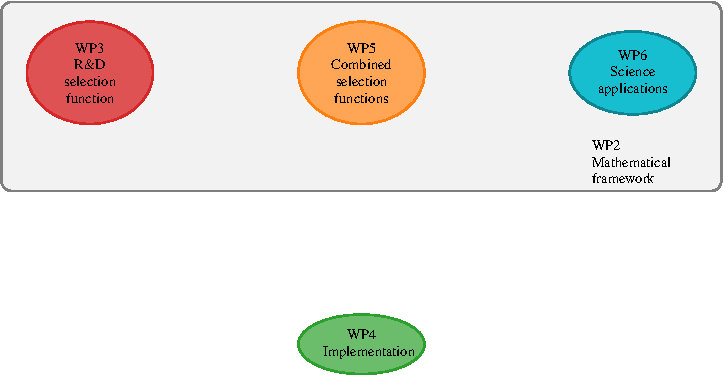
\includegraphics[width=\linewidth]{dependencies.pdf}
    \caption{The dependencies between the work packages in \acro.}
    \label{fig:dependencies}
\end{figure}

\section{Management structure, milestones and procedures}
\label{sec:management}

\subsection{Management}
\label{sec:mgtdetails}

The {\acro} consortium being relatively small the management structure can be kept simple in order to make the coordination of the efforts efficient. The management consists of three levels reflecting the structuring of the {\acro} work packages.
\begin{description}
    \item[Administrative management] This first level concerns the administrative management of {\acro}, including financial management and reporting to the European Commission. It is carried out by the {\acro} coordinator (A.~Brown) with the support of the Leiden Observatory institute management team.
    \item[Overall project management and coordination] This second level concerns the global scientific and technical control and coordination of the project, ensuring that the tasks are properly carried out and remain on schedule, and that the objectives of {\acro} are fulfilled. It is carried out by the \textbf{{\acro} executive board}, formed by the managers of the work packages: A.~Brown, R.~Drimmel, H.-W.~Rix, and V.~Belokurov. In order to keep communications within the consortium as efficient as possible the main contacts at NYU and MONA (D.~Hogg and A.~Casey) will have a standing invitation to attend the executive board meetings (see below).
    \item[Work package management] The third level of management concerns the main work packages. Each WP manager has the responsibility of supervising the execution of the core tasks assigned to their host institution, the work of the partners carrying out specific parts of the tasks attached to the work package, and report to the executive board accordingly.
    
    We do not further specify the management procedures for each work package beyond the items given in \secref{sec:procedures}, since the work in each of the work packages WP\ref{wp:selfundefinition} to WP\ref{wp:scienceappl} will be integrated in already existing and well established teams in each host institution.
\end{description}

This management structure together with the procedures described below is sufficient for a relatively small team spread over only six institutes working together closely in a scientific environment. Much of the coordination and supervision will take place through day-to-day contacts at the institutes involved and between institutes via e-mail and ad-hoc telecons. Similar structures were applied successfully to other EU-funded projects (FP7 GENIUS Collaborative project, FP7 GREAT Marie-Curie Initial Training Network) in which the coordinator was an active participant.

\subsection{Innovation management}
\label{sec:innovationmgmt}

The aim of {\acro} is to develop and deliver a new product (the Gaia selection function and tools to apply it) to the market of astronomy researchers. The wish for a selection function for the Gaia survey has been expressed on numerous occasions, meaning that this product will readily find a large user base. In order to uncover opportunities the astronomical community will be engaged during the lifetime of {\acro} through the availability of a prototype implementation of the Gaia selection function. The users thereof will be asked for feedback in the form of missing features or desired improvements. Community feedback wll also be obtained through presentation of {\acro} results at relevant scientific conferences.

\subsection{Procedures and reporting}
\label{sec:procedures}

We list here the procedures that will apply to the management of {\acro}:
\begin{itemize}
    \item The {\acro} coordinator will report to the European Commission following the rules applicable for research and innovation projects within the Horizon 2020 programme.
    \item {\acro} will hold at least three plenary meetings open to participation of all its members: the kick-off, mid-term, and closing meeting. The participation of the partner institute coordinators (or a representative) will be mandatory. Other plenary meetings may be held if needed.
    \item Specialized meetings or workshops will be organized on an `as-needed' basis by the WP managers.
    \item The executive board will hold teleconferences at least once a month to track the status of the tasks. The minutes of these teleconferences will be made available to the members of the consortium.
    \item The executive board shall ensure the coordination of the {\acro} work with the wider activities on the Gaia mission and its data releases, in particular ensuring the coordination with ESA and DPAC (see \secref{sec:dissemination-exploitation}). This can be done efficiently through membership of several {\acro} team members in DPAC.
\end{itemize}

\subsection{Consortium agreement}
\label{sec:cons_agreement}

The internal workings of {\acro} and the roles and responsibilities of the partners will be formalized through a consortium agreement will be drawn up and agreed at the start of the programme. It will define the decision taking procedures in {\acro} and the mechanisms for conflict resolution, which will be channelled through the Executive Board, as well as the management of intellectual property rights as described in \secref{sec:openipr}.

\subsection{Recruitment strategy}
\label{sec:recruit}

The recruitment policy for {\acro} will conform to the principles of the European Charter for Researchers and the Code of Conduct for their recruitment. It will take place in a globally coordinated way during the six-month setup phase described in \secref{sec:wptiming}, placing an emphasis on individual excellence and capacity for team working, while taking care to ensure equal opportunity and gender balance.

%%%%%%%%%%%%
% MILESTONES
%%%%%%%%%%%%

\milestone[1]{Kick-off meeting}{Organized by {\acro} executive board}{WP\ref{wp:management}}
\milestone[4]{Hiring of researchers}{Partners notify {\acro} executive board}{WP\ref{wp:management}}
\milestone[12]{Document on mathematical formulation of selection function submitted to peer-reviewed journal}{Document approved by {\acro} executive board}{WP\ref{wp:selfundefinition}}
\milestone[18]{Document describing the preliminary Gaia selection function.}{Document approved by {\acro} executive board}{WP\ref{wp:selfungaia}}
\milestone[21]{Mid-term meeting and community workshop}{Organized by {\acro} executive board}{WP\ref{wp:management}}
\milestone[24]{Public prototype of selection function implementation}{Software and data released and validated by user group}{WP\ref{wp:selfunimplementation}}
\milestone[36]{Papers and documentation describing the Gaia and combined selection functions ready to submit to peer-reviewed journals}{Verified by {\acro} executive board}{WP\ref{wp:selfungaia}, \ref{wp:selfunimplementation}, \ref{wp:selfuncombine}}
\milestone[41]{Closing meeting and community workshop}{Organized by {\acro} executive board}{WP\ref{wp:management}}
\milestone[42]{Publicly available selection function implementation, tools and data}{Software and data released and validated by user group}{WP\ref{wp:management}, \ref{wp:selfunimplementation}}

\makemilestoneslist

%%%%%%%
% RISKS
%%%%%%%
\criticalrisk{Late recruitment of researchers. Medium}{WP\ref{wp:selfungaia}--\ref{wp:scienceappl}}{Six month preparatory phase added in schedule to accommodate early advertizing of open positions. Use professional network of {\acro} participants. Executive board will track recruitment.}
\criticalrisk{Recruited researchers leaving early. Medium}{WP\ref{wp:selfungaia}--\ref{wp:scienceappl}}{Keep staff motivated, including through supporting career development. Coordinator and executive board will monitor personnel happiness.}
\criticalrisk{Unexpected complexity of tasks. High}{WP\ref{wp:selfungaia}--\ref{wp:scienceappl}}{Prioritize the {\acro} efforts and make timely decisions on dropping tasks deemed to complex.}
\criticalrisk{Lack of information from DPAC. Low}{WP\ref{wp:selfungaia}--\ref{wp:selfuncombine}}{{\acro} team members will be embedded in DPAC. Coordinator can identify alternative routes within DPAC to obtaining information.}
\criticalrisk{Coordination problems with ESA and DPAC leading to the selection function data products not being available through ESA archives. Low}{WP\ref{wp:selfunimplementation}}{Plan for alternative distribution channels. Coordinator to maintain close connections to ESA and DPAC.}
\criticalrisk{Delay of Gaia data releases. Can lead to difficulties in coordinating with DPAC/ESA (due to their prioritizing working on the releases). Medium}{WP\ref{wp:selfungaia}--\ref{wp:scienceappl}}{Coordinator to monitor the situation and agree mitigation measures with ESA/DPAC. We stress that even in the extremely unlikely case that no further Gaia data releases were to happen, the {\acro} effort will still have a large positive impact on the exploitation of the existing Gaia DR2 data.}

\makerisklist

\section{Consortium as a whole}
\label{sec:consortium}

The idea for this proposal grew out of discussions at several Gaia Sprints\footnote{\url{http://gaia.lol}} in which all of the {\acro} members participated, Hogg, Casey, Price-Whelan, and Fouesneau being members of the organizing team of the Sprints. In particular at the Gaia Sprint that took place in Santa Barbara (USA) in March 2019, two sessions were dedicated solely to discussing the Gaia selection function. It was concluded that only a significant and dedicated effort, specifically funded, could realistically lead to the construction of the Gaia selection function and the corresponding tools and data needed to use it.

The consortium represents a combination of Gaia/DPAC experts (Brown, Drimmel, Fouesneau), experts that have given much thought to the principles of selections functions and worked on aspects of the Gaia selection function (Hogg, Rix, Drimmel, Price-Whelan, Casey, Fouesneau). All the participants have undertaken scientific analyses of the Gaia data that clearly highlight the need for a selection function. \memo{Look up relevant publications.}
\begin{itemize}
    \item The Gaia expertise in the consortium is contributed by long-standing DPAC members who are deeply involved in the data processing for the Gaia mission. They provide expert insight into the detailed ingredients of the Gaia selection function and, more importantly, have an extensive network of contacts with experts in DPAC who can provide more detailed information where needed. The presence of the Gaia experts is crucial to the guidance of the researchers to be funded through {\acro}. We note that the other participants have extensive experience as users of Gaia data and thus bring an important complementary perspective to {\acro}.
    \item The expertise on the mathematical formulation of the selection function and on selection functions in general is essential to the success of {\acro}. The expertise stems from the actual construction of selection functions and applying these to analyses of a number of large surveys \memo{(Example citations)}.
    \item The requirements on a selection function and how it is provided in its practical form must be guided by the experience gained through advanced scientific analyses of data such as from the Gaia mission. The experience from successes and failures in past analyses will be very important in setting the priorities for the research \& development in {\acro}.
\end{itemize}

The partners from Australia and the USA contribute deep knowledge of selection function issues based on their past scientific work. Their perspective as experienced users of the Gaia data will be essential to ensure that the developments in {\acro} stay focused on satisfying the needs of the astronomical community in general, and not just the needs of DPAC experts.

The participants in {\acro} have a long track record of effective collaboration as can be seen from the many joint publications. In addition good connections exist to experts who have already taken concrete steps to providing a Gaia selection function implementation, such as Boubert \& Everall\footnote{\url{https://github.com/DouglasBoubert/selectionfunctions}} (Oxford, Cambridge) and Rybizki\footnote{\url{https://github.com/jan-rybizki/gdr2_completeness}} (Heidelberg). Through the organization of Gaia Sprints and other workshops\footnote{For example the Gaia DR2 Exploration Lab \url{https://www.cosmos.esa.int/web/gaia-dr2-exploration}.} the participants have a proven track record of engaging the astronomical community, an important aspect of making sure that the tools and data delivered by {\acro} fulfil actual user needs.

The coordinator, A.~Brown, is also a member of the management committee of the COST action CA18104 `Revealing the Milky Way with Gaia'\footnote{\url{http://www.mw-gaia.org/}} and is co-I on the recently submitted proposal for a Marie Sk\l{}odowska-Curie Innovative Training Network also called `Revealing the Milky Way with Gaia'. We foresee participation in the conferences organized through the MW-Gaia COST action as part of the dissemination activities and if the ITN proposal is successful we would offer training in the use of the Gaia selection to the PhD students in that network. This could take place for example at one of the schools planned by the ITN, or through participation of the PhD students in our planned community workshop. \memo{Add another communitt workshop, for example tied to the mid-term review?}

\section{Resources to be committed}
\label{sec:resources}

\makesummaryofefforttable

\costsTravel{ULEI}{2500}{Explain}
\costsEquipment{ULEI}{3000}{Not needed probably}
\costsOther{ULEI}{60000}{TBD}

\makecoststable

%%% Local Variables:
%%% mode: latex
%%% TeX-master: "proposal-main"
%%% End:
 % Section III

\bibliographystyle{aa}       %References go to end of Section III
\bibliography{refs}

\clearpage

\chapter{Members of the consortium}
\label{cha:members}

\instructions{
\textit{This section is not covered by the page limit.}
\vskip0.2cm
\textit{The information provided here will be used to judge the operational capacity. Please make sure that you do not include information here that relates to the headings under sections 1 to 3. Experts will be instructed to ignore any information here which appears to have been included to circumvent page limits applying to those section.}
}

\section{Participants (applicants)}
\label{sec:participants}

\instructions{
Please provide, for each participant, the following (if available):\\
\begin{itemize}
    \item a description of the legal entity and its main tasks, with an explanation of how its profile matches the tasks in the proposal;
    \item a curriculum vitae or description of the profile of the persons, including their gender, who will be primarily responsible for carrying out the proposed research and/or innovation activities; 
    \item a list of up to 5 relevant publications, and/or products, services (including widely- used data sets or software), or other achievements relevant to the  call content; 
    \item a list of up to 5 relevant previous projects or activities, connected to the subject of this proposal; 
    \item a description of any significant infrastructure and/or any major items of technical equipment, relevant to the proposed work; 
    \item if operational capacity cannot be demonstrated at the time of submitting the proposal, describe the concrete measures that will be taken to obtain it by the time of the implementation of the task.
\end{itemize}
}

\subsubsection{Universiteit Leiden}
\label{sec:ulei}

\paragraph{General description}
Leiden Observatory is the astronomy department at Leiden University, where world-class research is conducted covering areas of observational and theoretical astrophysics, instrumentation, and laboratory astrophysics. 
Leiden Observatory provides an environment where astronomers can be consulted directly on their wishes for the Gaia selection function and its practical implementation. At Leiden Observatory Undergraduate courses are given at all levels. The graduate programme currently involves 80 PhD students.

\paragraph{Key persons}
Dr.~Anthony Brown (male) is a faculty member of Leiden Observatory. He has published over 75 papers in the peer-reviewed literature, and supervised 9 PhD students and several postdocs. He has been deeply involved with the Gaia mission since 1997, having contributed to the optimization of the mission, the preparations for the data processing, and the implementation of several algorithms in the DPAC data processing pipelines. He currently serves as the chair of the Gaia Data Processing and Analysis Consortium and is a member of the Gaia Science Team. The efforts described in this proposal will very much benefit from the extensive expertise of Brown on both the Gaia spacecraft and its instruments as well as the DPAC processing pipelines. The close connections to ESA and DPAC through Brown's role in the latter will facilitate the communications regarding details of the selection function, the integration of the results in the Gaia archive, and the transfer of expertise to DPAC.

\paragraph{Relevant publications}
\begin{itemize}
    \item Gaia Collaboration, \textbf{Brown}, et al., 2018, Gaia Data Release 2. Summary of the contents and survey properties, A\&A 616, A1 
    \item Snellen \& \textbf{Brown}, 2018, The mass of the young planet Beta Pictoris b through the astrometric motion of its host star, Nature Astronomy 2, 883 
    \item Zari, Hashemi, \textbf{Brown}, et al., 2018, 3D mapping of young stars in the solar neighbourhood with Gaia DR2, A\&A 620, A172 
    \item  Luri, \textbf{Brown}, et al., 2018, Gaia Data Release 2. Using Gaia parallaxes, A\&A 616, A9 
    \item Helmi, Babusiaux, Koppelman, Massari, Veljanoski, \textbf{Brown}, 2018, The merger that led to the formation of the Milky Way's inner stellar halo and thick disk, Nature 563, 7729 
\end{itemize}

\paragraph{Relevant previous projects}
Brown was the main contact point at ULEI for the following projects:
\begin{itemize}
    \item FP6 ELSA Marie-Curie Research Training Network
    \item ESF GREAT Research Network Programme 
    \item FP7 GREAT Marie-Curie Initial Training Network
    \item FP7 GENIUS Collaborative project (SPA.2013.2.1-01 Exploitation of space science and exploration data)
    \item BIG-SKY-EARTH Trans Domain COST Action
\end{itemize}

\paragraph{Significant infrastructure}
Leiden Observatory shares a building with the Lorentz centre, an international centre for workshops in the sciences which offers excellent facilities for hosting workshops, conferences, and schools. In particular, office space is available for bringing researchers together for extended periods.
\newpage
\subsection{Max-Planck-Institut f\"ur Astronomie (MPIA)}
\label{sec:mpg}

\paragraph{General description}
MPIA is a large and leading research institution, with three departments 'Galaxies', 'Star and Planet Formation', and (as of 1.3.2020) 'Atmosphere Physics of Exoplanets'. Its research approaches encompass observation, instrumentation development, and theoretical modelling. MPIA has played a key role in Gaia (having led the DPAC CU8 development), and Gaia data are used across the institute: MPIA researches have over 150 refereed publications involving Gaia or Gaia data, since Gaia DR1. MPIA has a long-term staff of 25 members, and about 60 post-docs and 60 PhD students.

\paragraph{Key persons} 
Hans-Walter Rix is director of the 'Galaxies and Cosmology' department at MPIA,
and adjunct faculty at Heidelberg University. He has published over 500 peer-refereed papers (about 150 of them on the Milky Way or Gaia),
and over the last 20 years has supervised 15 students, and 30 post-docs.
He has held an ERC Advanced Grant on studying the dynamical structure of the Galactic disk, and is now the project scientist for the SDSS-V survey: the only survey to provide consistent all-sky, high-quality spectra of stars to complement Gaia. 

\paragraph{Relevant publications}
\begin{itemize}
    \item Xue, \textbf{Rix} et al., 2008, ApJ, 684, 1143 (527 cit), Milky Way's Dark Matter Halo Mass
    \item Bovy \& \textbf{Rix}, 2013, ApJ, 779, 115 (290 cit) A Direct Dynamical Measurement of the Milky Way's Disk Surface Density Profile, Disk Scale Length, and Dark Matter Profile 
    \item \textbf{Rix} \& Bovy, 2013, A\&A Review, 21, 61 (165 cit.) Mapping and modeling the Galactic disk
    \item Eilers, Hogg \& \textbf{Rix}, 2019, ApJ, 871, 120E (51 cit.) The Circular Velocity Curve of the Milky Way from 5 to 25 kpc
    \item El-Badry \& \textbf{Rix} , 2019, MNRAS, 489, 5822 (13 cit.) Gaia discovery of an equal-mass `twin' binary population reaching 1000 + au separations
\end{itemize}

\paragraph{Relevant previous project}
\begin{itemize}
    \item FP7-PEOPLE-2007-1-1-ITN
    \item ERC-2012-ADG-20120216
    \item FP7-INFRASTRUCTURES-2012-1
\end{itemize}

\paragraph{Significant infrastructure}
MPIA employs >100 PhD and PostDoc students: for them it offers 
a rich and structured research environment, a mentorng system
and career development. MPIA has priviledged access to MPG supercomputing resources,
and has extensive in-house computing. MPIA can host (also extended) workshop, from days to weeks, and from 5 to 100 persons. MPIA has extensive access to facilities for Gaia follow-up observations.



\newpage
\subsection{INAF - Osservatorio Astrofisico di Torino}
\label{sec:inaf}

\paragraph{General description}

The Istituto Nazionale di Astrofisica (INAF) promotes, coordinates, and carries out, within the context of programs of the European Union and other International Entities, research activities in the fields of Astronomy, Radioastronomy, Space Astrophysics, and Cosmic Physics, in collaboration with Italian Universities as well as other private and public, national and international research organizations. In particular, INAF coordinates research activities carried out at national facilities (the Telescopio Nazionale Galileo, TNG, in the Canary Islands, and the Large Binocular Telescope, LBT, on Mt. Graham, Arizona) and at 18 research institutes and astronomical observatories on Italian soil. The proposed project will be undertaken at the Osservatorio Astrofisico di Torino (OATo), one of the INAF institutes. 

\paragraph{Key persons}

Dr.~Ronald Drimmel (male) is a research astronomer (staff) of INAF whose research interest is primarily the structure and dynamics of the Milky Way, especially the investigation of non-axisymmetric structures such as the spiral arms and the warp. While currently he works with Gaia data, he has analysed infrared and far-infrared all-sky data from the COBE satellite to derive a model of the distribution of the stars and interstellar dust in the Milky Way on large scales. Drimmel has been a key member of the Gaia Data Processing and Analysis Consortium (DPAC), serving as it's Deputy Chair from 2006 to 2012. Currently he is contributing to the construction of an all-sky map of the total Galactic extinction. Drimmel is also on the Gaia Payload Experts group, responsible for monitoring and evaluating the performance of the Gaia instrument.

Dr.~Richard Smart (male) has been active in Gaia since it's conception. He was the provider of the Initial Gaia Source List \cite{2014A&A...570A..87S} and is member of the Gaia Ultra Cool Dwarf and Gaia Ground Based Tracking work package and is leading the effort to produce the Gaia Catalogue of Nearby Stars that contains all stars to M9 within 100~pc of the Sun. Smart was the coordinator of the EU FP7 RISE program Interpretation and Parameterization of Extremely COOL objects (IPERCOOL, 247593), the Italian coordinator for the GENIUS  program and has managed 5 postdocs at the Observatory. 

Dr.~Alessandro Spagna (male) is a senior research astronomer (staff) of INAF. His main scientific interests are in the field of ground-based and space astrometry, in the construction of wide field surveys for the study of the Galactic stellar populations and the chemo-dynamical evolution of the Milky Way. In particular his research activity focuses on the formation of the Galactic thick disc and stellar halo. He has been also involved in various projects for the construction of all-sky catalogues, such as Hipparcos, Guide Star Catalog II, and Gaia. 


\paragraph{Relevant publications}
\begin{itemize}
    \item Poggio, \textbf{Drimmel}, et. al., 2020, Evidence of a dynamically evolving Galactic warp, Nature Astronomy (doi:10.1038/s41550-020-1017-3)
    \item Poggio, \textbf{Drimmel}, et. al., 2018, The Galactic warp revealed by Gaia DR2 kinematics, MNRAS Letters 481, L21
    \item  Gaia Collaboration, Katz, Antoja, Romero-G\'omez, \textbf{Drimmel}, et al., 2018 Gaia Data Release 2. Mapping the Milky Way disc kinematics A\&A 616, A11
    \item \textbf{Drimmel} \& Spergel, 2001, Three-dimensional Structure of the Milky Way Disk: The Distribution of Stars and Dust beyond 0.35~$R_\mathrm{solar}$ ApJ, 556, 181
    \item \textbf{Drimmel}, 2000, Evidence for a two-armed spiral in the Milky Way A\&A, 358, L13
\end{itemize}

\paragraph{Relevant previous projects}

Drimmel was the main contact point at INAF for the following past projects:
\begin{itemize}
    \item FP6 ELSA Marie-Curie Research Training Network
\end{itemize}
Drimmel also participated in the following EU funded projects: 
\begin{itemize}
    \item ESF GREAT Research Network Programme 
    \item FP7 GREAT Marie-Curie Initial Training Network
    \item FP7 GENIUS Collaborative project (SPA.2013.2.1-01 Exploitation of space science and exploration data)
\end{itemize}


\paragraph{Significant infrastructure}

In the context of this proposal, the most relevant facilities that INAF participants have access to is the Marconi supercomputer at the CINECA, a national high-performance computing centre. Marconi is classified in Top500 list among the most powerful supercomputer:  rank 12 in November 2016, and rank 19 in the November 2019 list. Also available is an Oracle Database Machine at Trieste Observatory.
\newpage
\subsection{Institute of Astronomy at the University of Cambridge (UCAM)}
\label{sec:ucam}

\paragraph{General description}

Institute of Astronomy (IoA) is one of the three Astronomy departments at the University of Cambridge, the other two being Cavendish Astrophysics Group and the Astrophysics Group at the Department of Applied Mathematics and Theoretical Physics. The IoA has 18 permanent staff members, some 100 postdoctoral fellows, approximately 50 graduate students and 25 support staff. The Institute also hosts the Cambridge Astronomical Survey Unit, the DPAC Coordination Unit 5 in charge of Photometric Processing and the Gaia-ESO survey. The Institute’s research portfolio includes the full spectrum of the cutting edge Astrophysics topics, from the Early Universe to Exo-planets and instrument design and construction. The Institute played a uniquely active role in the scientific exploration of the Gaia DR1 and DR2 resulting in more than 200 publications by the IoA members (over the last 4 years only). The direct daily interface between the broad and active research body and CASU and CU5 makes UCAM an especially attractive environment for the proposed project.


\paragraph{Key persons}

Prof.~Vasily Belokurov (male) is a Professor of Astronomy at the University of Cambridge. He is a survey scientist, whose expertise is in data mining, galactic dynamics and machine learning. The broad theme of his research is galaxy formation and evolution, with a particular focus on the Milky Way halo, low-mass galaxies and local constraints on Dark Matter. Belokurov has supervised more than 20 graduate students and worked closely with an appreciable number of postdocs. He has published more than 250 papers in refereed journals. It is worth mentioning separately the papers that present the analysis based on the data from the ESA’s Gaia mission. Gaia Data Release 1 was delivered in 2016, while the Gaia DR2 arrived less than 2 year ago. So far, Belokurov has published $>$40 papers in refereed journals, relying on either Gaia DR1 or DR2 data.

Andrew Everall (male) is a PhD student at the Institute of Astronomy working with supervisors Prof.~Vasily Belokurov and Prof.~Wyn Evans. His core focus is on constraining the Milky Way Dark Matter distribution and specifically the local DM density. He has worked significantly on selection functions for multi fibre spectrographs and has already performed a substantial amount of work on selection functions for Gaia DR2 and subsets therein with Dr.~Douglas Boubert. 

\paragraph{Relevant publications}

\begin{itemize}
    \item Boubert \& \textbf{Everall}, submitted, Completeness of the \textit{Gaia}-verse II: what are the odds that \textit{Gaia} DR2 missed a star?
    \item Boubert, \textbf{Everall} \& Holl, submitted, Completeness of the Gaia-verse I: when was Gaia’s eye off the sky?
    \item Grady, \textbf{Belokurov} \& Evans, 2020, MNRAS, 492, 3128, Age demographics of the Milky Way disc and bulge
    \item Deason, \textbf{Belokurov} \& Sanders, 2020, MNRAS, 490, 3426, The total stellar halo mass of the Milky Way
    \item \textbf{Everall} \& Das, 2020, MNRAS, 493, 2042, seestar: Selection functions for spectroscopic surveys of the Milky Way
    \item \textbf{Everall}, Evans, \textbf{Belokurov}, Schönrich, 2019, MNRAS, 489, 910, The tilt of the local velocity ellipsoid as seen by Gaia
    \item Erkal, \textbf{Belokurov}, et al., 2019, MNRAS, 487, 2685, The total mass of the Large Magellanic Cloud from its perturbation on the Orphan stream
    \item Torrealba, \textbf{Belokurov}, et al., 2019, MNRAS, 488, 2743, The hidden giant: discovery of an enormous Galactic dwarf satellite in Gaia DR2
    \item Necib, Lisanti, \textbf{Belokurov}, 2019, ApJ, 874, 3
    \item \textbf{Belokurov}, Erkal, 2019, MNRAS, 482, L9
    \item \textbf{Belokurov} et al., 2018, MNRAS, 478, 611, Co-formation of the disc and the stellar halo
\end{itemize}

\paragraph{Relevant previous projects}

\begin{itemize}
    \item Starting Grant (StG), PE9, ERC-2012-StG\_20111012
    \item Gaia-ESO survey. A large European survey which was specifically aimed at collecting spectroscopic data complementary to the Gaia mission.
\end{itemize}

\paragraph{Significant infrastructure}
\newpage
\subsection{Monash University}
\label{sec:mona}

\paragraph{General description}
Monash University is a world-class teaching and research institution located in Melbourne, Australia. The School of Physics \& Astronomy at Monash University includes researchers spanning observational and theoretical astrophysics, with focussed groups on exoplanets, binary stars, stellar astrophysics, galactic structure, gravitational waves, and more. Statistical inference and data analysis are common to all of these research groups, making Monash University an excellent place to host researchers who are developing the Gaia selection function and applying it to key areas in astrophysics.

\paragraph{Key persons}
Dr.~Andrew Casey (male) is a faculty member at Monash University and an Australian Research Council DECRA Fellow. He is currently six years post-PhD and has an extensive track record of high-quality peer-reviewed publications: $>$100 publications that have accrued 5,988 citations, yielding a h-index of 34 and a m-index of 3.4. Casey is a co-organiser of the Gaia Sprints workshops (2016--2019, inclusive), which have helped strengthen the astrophysics community who are working with Gaia data.


\paragraph{Relevant publications}
\begin{itemize}
	\item \tetxbf{Casey}, et al., 2019, A Data-driven Model of Nucleosynthesis with Chemical Tagging in a Lower-dimensional Latent Space, 2019, ApJ, 887, 73
	\item \textbf{Casey}, et al., 2019, Tidal Interactions between Binary Stars Can Drive Lithium Production in Low-mass Red Giants, 2019, ApJ, 880, 125
	\item Simpson, Martell, Da Costa, \textbf{Casey}, et al., 2019, The GALAH survey: co-orbiting stars and chemical tagging, MNRAS, 482, 5302
	\item Williams, Belokurov, \textbf{Casey}, Evans, 2017, On the run: mapping the escape speed across the Galaxy with SDSS, MNRAS, 468, 2359
	\item \textbf{Casey} et al., 2017, The RAVE-on Catalog of Stellar Atmospheric Parameters and Chemical Abundances for Chemo-dynamic Studies in the Gaia Era, ApJ, 840, 59
\end{itemize}

\paragraph{Relevant previous projects}

\begin{itemize}
    \item Gaia-ESO survey. A large European survey which was specfically aimed at collecting spectrocopic data complementary to the Gaia mission.
\end{itemize}

\paragraph{Significant infrastructure}
As of 2020 Monash University joins the Australian Research Council Centre of Excellence in Astrophysics in 3-Dimensions (ASTRO 3D), a \$30\,M AUD (18.3\,M Euro) initiative for astrophysics research in Australia. This initiative includes researchers working on the formation and evolution of the Milky Way galaxy, single and binary star evolution, and other key science goals for the Gaia mission. The Australian-led GALAH survey is one of the key projects of ASTRO 3D, with the goal to obtain high-resolution optical spectra for up to $\sim10^6$ stars. Currently the GALAH/Gaia sub-sample represents the highest quality set of stars with precise astrometry and chemical abundance information. This provides a unique opportunity to study the chemo-dynamical history of the Milky Way in exquisite detail, yet the Gaia and GALAH samples are both subject to selection function effects. Monash University is the ideal place for researching binary population inference with the Gaia selection function, and the complement of the Gaia selection functions with other surveys (e.g. GALAH).

\newpage
\subsection{New York University}
\label{sec:nyu}

\paragraph{General description}

The Department of Physics at New York University hosts 36 tenure and tenure-track professors, two clinical faculty members, a few dozen research scientists and postdoctoral fellows, and over 80 graduate and 90 undergraduate students. The majority of the faculty are engaged in cutting-edge research in astrophysics and cosmology, particle and astro-particle experimental and theoretical physics, hard and soft condensed matter physics, biophysics, fluid dynamics, and applied mathematical physics.

\paragraph{Key persons}
Prof.~David W.~Hogg (male) is Professor of Physics and Data Science in the Center for Cosmology and Particle Physics in the Department of Physics. He is also Group Leader for the Astronomical Data Group in the Center for Computational Astrophysics of the Flatiron Institute, a staff member in the Centre for Data Science at New York University, and he has an affiliation with the Max-Planck-Institut für Astronomie. His main research interests are in observational cosmology, especially approaches that use galaxies to infer the physical properties of the Universe. He also works on the properties and kinematics of stars in the Galaxy, and the measurement and discovery of planets around other stars. In all areas, he is interested in developing the engineering systems that make these projects possible. He has published 250 peer-reviewed publications and has supervised or co-supervised 11 PhD students and numerous postdoctoral researchers. He is the chair of the organising committee for all Gaia Sprints held to date.

Dr.~Adrian Price-Whelan (male) is a postdoctoral fellow at the Center for Computational Astrophysics at the Flatiron Institute. His main research centres on the structure and formation of the Milky Way. His analysis of the GD-1 stream in the Gaia DR2 data led to the discovery of gaps along the stream which could point to the presence of dark matter substructures in the halo of the Milky Way\cite{2018ApJ...863L..20P,2019ApJ...880...38B}. This work was also one of the triggers of the discussions on the need for a Gaia selection function. Price-Whelan is a major contributor to Astropy \cite{astropy2018}, which is the eco-system in which the {\acro} tools are likely to be embedded. Price-Whelan is a co-organizer of the Gaia Sprint workshops.

\paragraph{Relevant publications}
\begin{itemize}
    \item Bonaca, \textbf{Hogg}, \textbf{Price-Whelan}, et al., 2019, The Spur and the Gap in GD-1: Dynamical Evidence for a Dark Substructure in the Milky Way Halo, ApJ, 880, 38
    \item Anderson, \textbf{Hogg}, et al., 2018, Improving Gaia Parallax Precision with a Data-driven Model of Stars, AJ, 156, 145
    \item Bonaca \& \textbf{Hogg}, 2018, The Information Content in Cold Stellar Streams, ApJ, 867, 101
    \item Eilers, \textbf{Hogg}, Rix, \& Ness, 2019, The Circular Velocity Curve of the Milky Way from 5 to 25 kpc, ApJ, 871, 120
    \item Rezaei Kh, Bailer-Jones, \textbf{Hogg}, et al., 2018, Detection of the Milky Way spiral arms in dust from 3D mapping, A\&A, 618, 168
    %\item \textbf{Price-Whelan} \& Bonaca, 2018, Off the Beaten Path: Gaia Reveals GD-1 Stars outside of the Main Stream, ApJ, 863
    %\item Astropy Collaboration; \textbf{Price-Whelan}, et al., 2018, The Astropy Project: Building an Open-science Project and Status of the v2.0 Core Package, AJ, 156, 123
    %\item \textbf{Price-Whelan}, et al., 2019, Discovery of a Disrupting Open Cluster Far into the Milky Way Halo: A Recent Star Formation Event in the Leading Arm of the Magellanic Stream?, ApJ, 887, 19
\end{itemize}

\paragraph{Relevant previous projects}
\begin{itemize}
    %NSF Astronomy and Astrophysics Research Grant AST-1517237, New Probabilistic Methods for Observational Cosmology; NSF Cyber-Enabled Discovery Type I Grant (IIS-1124794), A Unifored Probabilistic Model of Astronomical Imaging; NASA HST Archival Research Grant (AR-13250), Probabilistic Self-calibration of the WFC3 IR Channel; NSF Astronomy and Astrophysics Research Grant (AST-0908357), Dynamical models from kinematic data: The Milky Way Disk and Halo
    \item NSF Astronomy and Astrophysics Research Grant AST-1517237, New Probabilistic Methods for Observational Cosmology
    \item NSF Cyber-Enabled Discovery Type I Grant (IIS-1124794), A Unified Probabilistic Model of Astronomical Imaging
    \item NASA HST Archival Research Grant (AR-13250), Probabilistic Self-calibration of the WFC3 IR Channel
    \item NSF AST-0908357, Dynamical models from kinematic data: The Milky Way Disk and Halo
\end{itemize}

\paragraph{Significant infrastructure}
New York University and the Flatiron Institute are both located in New York City. Together these institutes host hundreds of visiting researchers every year and the Flatiron Institute has been host for multiple Gaia Sprints in the past, offering a unique and collaborative space that cultivates a lively atmosphere for research.
Hogg has strong collaborations with astrophysicists and data scientists from all research institutions in the New York area.

\newpage

\section{Third parties involved in the project (third party resources)}
\label{sec:third-parties}

\instructions{
\textit{Please complete, for each participant, the following table (or simply state "No third parties involved", if applicable).}}

\begin{tabular}{|p{.8\textwidth}|p{.1\textwidth}|}
  \hline  
  \multicolumn{2}{|l|}{\cellcolor[gray]{0.8}\textbf{ULEI}}\\
  \hline
  Does the participant plan to subcontract certain tasks (please note that core tasks of the project should not be sub-contracted) &
  \textbf{Y/N} \\
  \hline
Does the participant envisage that part of its work is performed by linked
third parties &
  \textbf{Y/N} \\
  \hline
  Does the participant envisage the use of contributions in kind provided by
third parties (Articles 11 and 12 of the General Model Grant Agreement) &
  \textbf{Y/N}\\
  \hline
\end{tabular}

\begin{tabular}{|p{.8\textwidth}|p{.1\textwidth}|}
  \hline  
  \multicolumn{2}{|l|}{\cellcolor[gray]{0.8}\textbf{MPG}}\\
  \hline
  Does the participant plan to subcontract certain tasks (please note that core tasks of the project should not be sub-contracted) &
  \textbf{Y/N} \\
  \hline
Does the participant envisage that part of its work is performed by linked
third parties &
  \textbf{Y/N} \\
  \hline
  Does the participant envisage the use of contributions in kind provided by
third parties (Articles 11 and 12 of the General Model Grant Agreement) &
  \textbf{Y/N}\\
  \hline
\end{tabular}

\begin{tabular}{|p{.8\textwidth}|p{.1\textwidth}|}
  \hline  
  \multicolumn{2}{|l|}{\cellcolor[gray]{0.8}\textbf{INAF}}\\
  \hline
  Does the participant plan to subcontract certain tasks (please note that core tasks of the project should not be sub-contracted) &
  \textbf{Y/N} \\
  \hline
Does the participant envisage that part of its work is performed by linked
third parties &
  \textbf{Y/N} \\
  \hline
  Does the participant envisage the use of contributions in kind provided by
third parties (Articles 11 and 12 of the General Model Grant Agreement) &
  \textbf{Y/N}\\
  \hline
\end{tabular}

\begin{tabular}{|p{.8\textwidth}|p{.1\textwidth}|}
  \hline  
  \multicolumn{2}{|l|}{\cellcolor[gray]{0.8}\textbf{UCAM}}\\
  \hline
  Does the participant plan to subcontract certain tasks (please note that core tasks of the project should not be sub-contracted) &
  \textbf{Y/N} \\
  \hline
Does the participant envisage that part of its work is performed by linked
third parties &
  \textbf{Y/N} \\
  \hline
  Does the participant envisage the use of contributions in kind provided by
third parties (Articles 11 and 12 of the General Model Grant Agreement) &
  \textbf{Y/N}\\
  \hline
\end{tabular}

\begin{tabular}{|p{.8\textwidth}|p{.1\textwidth}|}
  \hline  
  \multicolumn{2}{|l|}{\cellcolor[gray]{0.8}\textbf{MONA}}\\
  \hline
  Does the participant plan to subcontract certain tasks (please note that core tasks of the project should not be sub-contracted) &
  \textbf{Y/N} \\
  \hline
Does the participant envisage that part of its work is performed by linked
third parties &
  \textbf{Y/N} \\
  \hline
  Does the participant envisage the use of contributions in kind provided by
third parties (Articles 11 and 12 of the General Model Grant Agreement) &
  \textbf{Y/N}\\
  \hline
\end{tabular}

\begin{tabular}{|p{.8\textwidth}|p{.1\textwidth}|}
  \hline  
  \multicolumn{2}{|l|}{\cellcolor[gray]{0.8}\textbf{NYU}}\\
  \hline
  Does the participant plan to subcontract certain tasks (please note that core tasks of the project should not be sub-contracted) &
  \textbf{Y/N} \\
  \hline
Does the participant envisage that part of its work is performed by linked
third parties &
  \textbf{Y/N} \\
  \hline
  Does the participant envisage the use of contributions in kind provided by
third parties (Articles 11 and 12 of the General Model Grant Agreement) &
  \textbf{Y/N}\\
  \hline
\end{tabular}

%%% Local Variables:
%%% mode: latex
%%% TeX-master: "proposal-main"
%%% End:
 % Section IV
\chapter{Ethics and Security}
\label{cha:ethics}
\instructions{
\textit{This section is not covered by the page limit.}
}

\section{Ethics}
\label{sec:ethics}
\instructions{
If you have entered any ethics issues in the ethical issue table in the administrative proposal forms, you must:
\begin{itemize}
\item submit an ethics self-assessment, which:
\begin{itemize}
\item describes how the proposal meets the national legal and ethical requirements of the country or countries where the tasks raising ethical issues are to be carried out; 
\item explains in detail how you intend to address the issues in the ethical issues table, in particular as regard:
\begin{itemize}
\item research objectives (e.g. study of vulnerable populations, dual use, etc.)
\item research methodology (e.g. clinical trials, involvement of children and related consent procedures, protection of any data collected, etc.) 
\item the potential impact of the research (e.g. dual use issues, environmental damage, stigmatisation of particular social groups, political or financial retaliation, benefit-sharing, misuse, etc.).
\end{itemize}
\end{itemize}
\item provide the documents that you need under national law(if you already have them), e.g.:
\begin{itemize}
\item an ethics committee opinion;
\item the document notifying activities raising ethical issues or authorising such activities;
\end{itemize}
\end{itemize}
\textit{\indent If these documents are not in English, you must also submit an English summary of them (containing, if available, the conclusions of the committee or authority concerned).}
\vskip0.2cm
\textit{If you plan to request these documents specifically for the project you are proposing, your request must contain an explicit reference to the project title.}
}

{\acro} is a project devoted to research and development that will lead to data products and tools to apply selection functions to the analysis of data collected by a space astrophysics mission and other surveys. Hence, no ethics issues are expected to arise in the project. This is indicated in the form filled out online in the Funding \& tender opportunities portal. Specific clarifications:
\begin{itemize}
    \item Research and development in {\acro} is conducted on publicly available data from astronomical surveys and we will make use as well of information from the Gaia Data Processing and Analysis Consortium to which the coordinator and several participants have access (as members of DPAC). For the participants who are not members of DPAC but need access to its non-public information a standard non-disclosure agreement (NDA) already exists which the participants in question will sign. In particular we stress:
    \begin{itemize}
        \item the research, development, and implementation of tools proposed here do not involve humans participants, human tissue, human embryos/foetuses, cells, or animals.
        \item no personal data is collected or processed for the purpose of the effort proposed.
    \end{itemize}
    \item Two third countries are involved, Australia and the United States of America.
    \begin{itemize}
        \item They will participate in the {\acro} research, development, and implementation of tools. As such they will only be working the publicly available data mentioned above and any code written by these partners will become part of the {\acro} tools that will be made publicly available.
        \item No personal data will be imported from or exported to the non-EU partners.
        \item No activities will be undertaken by the non-EU partners that are prohibited in the EU.
        \item Any data exchange with the non-EU partners will only involve publicly available data to which the non-EU partners already have access. In case DPAC information needs to be exchanged the NDA referred to above will also be applied to the non-EU partners.
    \end{itemize}
    \item The purpose of {\acro} is to advance astronomical research by enabling a much more advanced use of Gaia and other survey data than is possible today. Hence the focus of the efforts proposed here are exclusively civilian.
\end{itemize}

\section{Security}
\label{sec:security}
\begin{itemize}
\item Activities or results raising security issues: NO
\item ``EU-classified information'' as background or results: NO
\end{itemize}

%%% Local Variables:
%%% mode: latex
%%% TeX-master: "proposal-main"
%%% End: % Section V

%\appendix

%%% Proposal appendix % Appendix

%\backmatter

\end{document}
